
\chapter{Introduction}

% https://lilianweng.github.io/posts/2018-02-19-rl-overview/

\section{Sequential decision making}

\keywordDef{Reinforcement learning}
or \keywordDef{RL} is a class of methods for solving
various kinds of sequential decision making tasks.
In such tasks, we want to design an  \keywordDef{agent}
that interacts with an external \keywordDef{environment}.
  The agent maintains an internal state $s_t$, which it passes to its \keywordDef{policy}
  $\pi$ to choose an action $a_{t}=\pi(s_t)$.
  The environment responds by sending back an observation $o_{t+1}$,
  which the agent uses to update its internal state using the state-update
  function $s_{t+1}=U(s_t,a_{t},o_{t+1})$.
  See \cref{fig:agentEnv} for an illustration.


\subsection{Problem definition}
  
The goal of the agent is to choose a policy $\pi$ so as to
maximize the sum of expected rewards:
\be
V_{\pi}(s_0) = \expectQ{\sum_{t=0}^T R(s_t,a_t) |s_0}{p(a_0,s_1,a_1,\ldots,a_T,s_T|s_0,\pi)}
\label{eqn:valueFn}
\ee
where $s_0$ is the agent's initial state,
$R(s_t,a_t)$ is the \keywordDef{reward function} that the agent
uses to measure the value of performing an action in a given state,
$V_{\pi}(s_0)$ is the \keywordDef{value function} for  policy $\pi$ evaluated at $s_0$,
and the expectation is wrt
\begin{align}
p(a_0,s_1,a_1,\ldots,a_T,s_T|s_0,\pi)
&= \pi(a_0|s_0) \penv(o_1|a_0) \delta(s_1=U(s_0,a_0,o_1))  \\
& \times \pi(a_1|s_1) \penv(o_2|a_1,o_1) \delta(s_2=U(s_1,a_1,o_2)) \\
& \times \pi(a_2|s_2) \penv(o_3|a_{1:2},o_{1:2}) \delta(s_3=U(s_2,a_2,o_3)) 
\ldots
\label{eqn:distrib}
\end{align}
where $\penv$ is the environment's distribution over observations 
(which  is usually  unknown).
We define the optimal policy as
\be
\pi^* = \arg\max_{\pi} \expectQ{V_{\pi}(s_0)}{p_0(s_0)}
\ee
Note that picking a policy to maximize the sum of expected rewards is an instance
of the  \keywordDef{maximum expected utility} principle.
There are  various ways to design or learn an optimal policy,
depending on the assumptions we make about the environment,
and the form of the agent. We will discuss some of these options below.

\begin{figure}
\centering
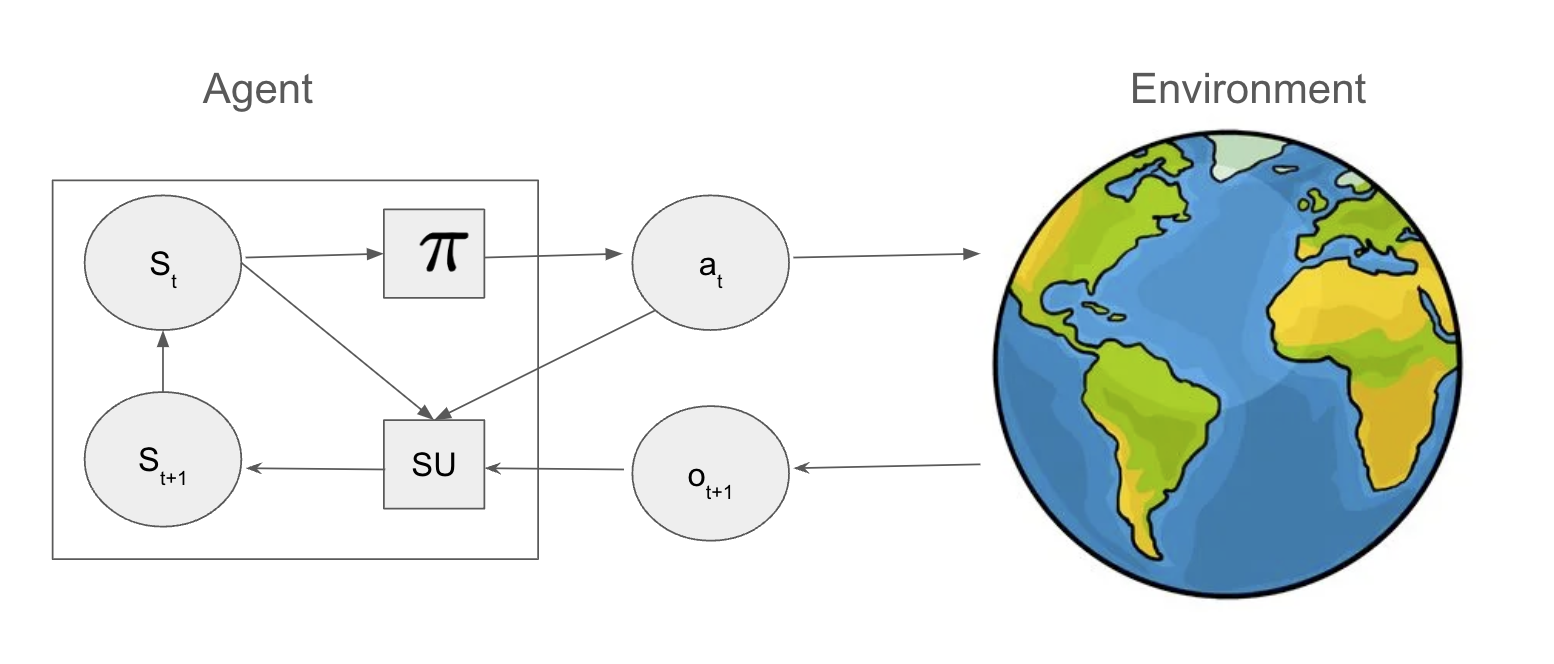
\includegraphics[height=2in]{figs/agentEnvSlide.png}
\caption{
  A small agent interacting with a big external world.
  }
\label{fig:agentEnv}
\end{figure}

\subsection{Universal model}
\label{sec:universal}

\begin{figure}
\centering
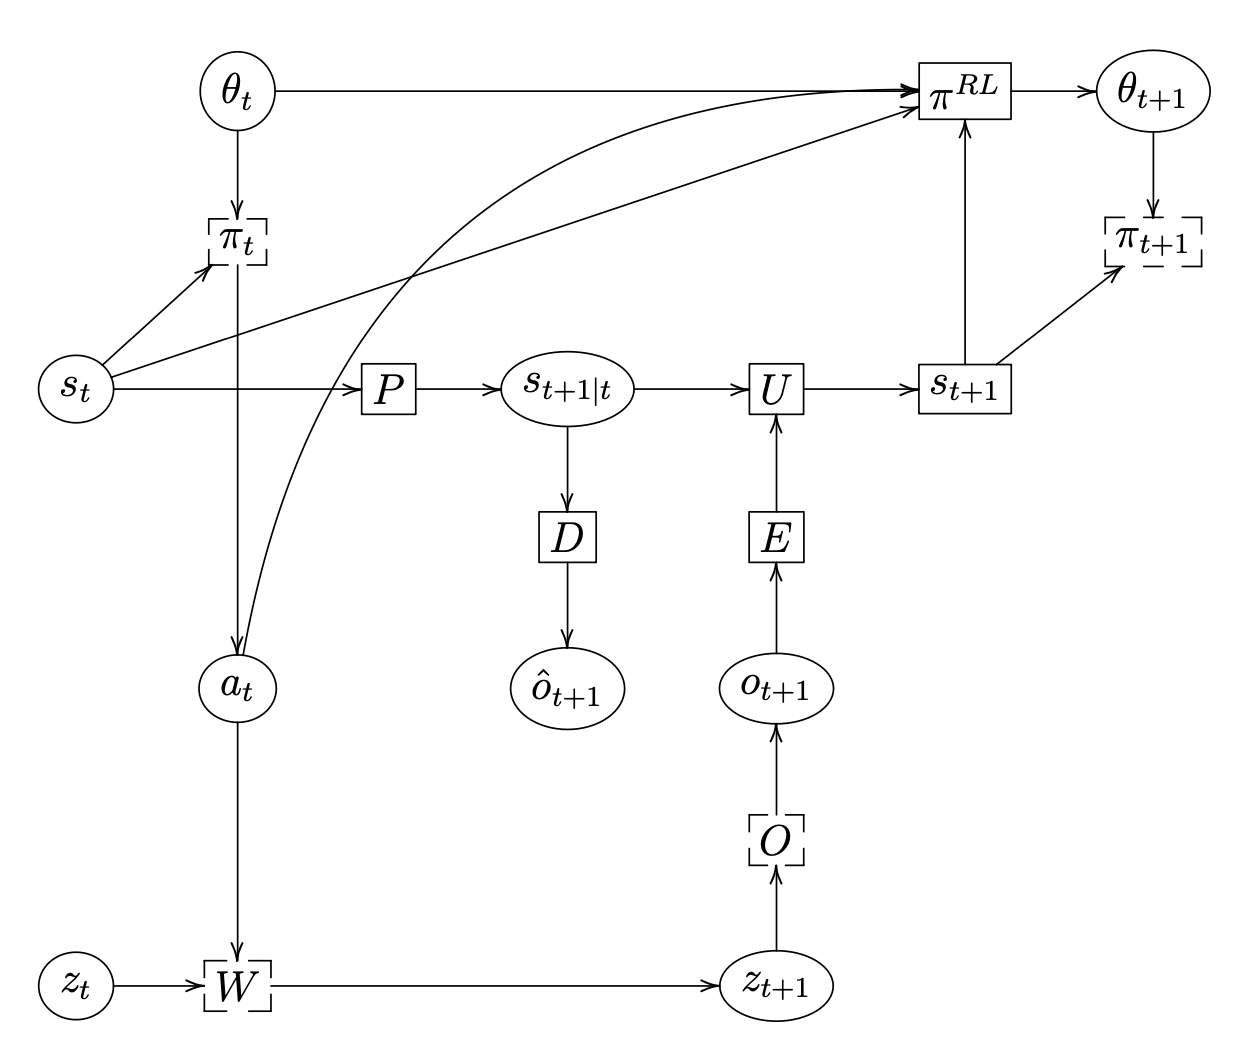
\includegraphics[height=3.5in]{figs/agentPGM2cropped}
\caption{
  Diagram illustrating the interaction of the agent and environment.
  The agent has internal state $s_t$, and chooses action $a_t$
  based on its policy $\pi_t$.
  It then predicts its next internal states, $s_{t+1|t}$, via
  the predict function $P$,
  and optionally predicts the resulting observation,
  $\hat{o}_{t+1}$, via the observation decoder $D$.
  The environment has (hidden) internal state $z_t$, which gets updated
  by the world model $W$ to give the new state $z_{t+1}=W(z_t,a_t)$
  in response to the agent's action.
  The environment also emits an observation $o_{t+1}$ via
  the observation model $O$.
  This gets encoded to $e_{t+1}$ by the agent's observation encoder $E$,
  which the agent uses to update its internal state using
  $s_{t+1}=U(s_t,a_t,e_{t+1})$.
  The policy is parameterized by $\theta_t$,
  and these parameters may be updated (at a slower time scale) by the RL
  policy $\pi^{RL}$.
  Square nodes are functions, circles are variables (either random or deterministic).
  Dashed square nodes are stochastic functions that take an extra source of randomness
  (not shown).
  }
\label{fig:POMDP}
\end{figure}


A generic representation for sequential decision making problems
(which is an extended version of the ``universal modeling framework'' proposed in
\citep{Powell2022}) is shown in \cref{fig:POMDP}.
Here we have assumed the environment can be modeled by a  controlled
\keywordDef{Markov process}\footnote{
%
The Markovian assumption is without loss of generality,
since we can always condition on the entire past sequence of states
by suitably expanding the Markovian state space.
} %
with hidden state $z_t$, which gets updated at each step in response
to the agent's action $a_t$.
To allow for non-deterministic dynamics, we write this as 
 $z_{t+1}=W(z_t,a_t,\epsilon^z_t)$,
where
$W$ is the environment's state transition function (which is usually not
known to the agent)
and
$\epsilon^z_t$ is random system noise.\footnote{
%
Representing a stochastic function as a deterministic function with some noisy
inputs is known as a functional causal model,
or structural equation model.
This is standard practice in the control theory and causality communities.
},
The agent does not see the world state $z_t$, but instead
sees a potentially noisy and/or partial observation $o_{t+1}=O(z_{t+1},\epsilon^o_{t+1})$ at each step,
where $\epsilon^o_{t+1}$ is random observation noise.
For example, when navigating a maze, the agent may only see what is in front of it,
rather than seeing everything in the world all at once;
furthermore, even the current view may be corrupted by sensor noise.
Any given image, such as one containing a door, could correspond to many
different locations in the world (this is called \keywordDef{perceptual aliasing}),
each of which may require a different action.
Thus the agent needs use  these observations to incrementally
update its own internal \keywordDef{belief state}
about the world,
using the state update function $s_{t+1}=SU(s_t,a_t,o_{t+1})$;
this represents the agent's beliefs about the underlying world state $z_t$,
as well as the unknown world model $W$ itself (or some proxy thereof).
In the simplest setting, the internal $s_t$ can just store all the past observations,
$\vh_t=(\vo_{1:t},\va_{1:t-1})$, but such non-parametric models
can take a lot of time and space to work with, so we will usually
consider parametric approximations.
The agent can then pass its state to its policy to pick actions,
using
$a_{t+1}=\pi_t(s_{t+1})$.


We can further elaborate the behavior of the agent by breaking the state-update
function into two parts.
First the agent predicts its own next state, $s_{t+1|t}=P(s_t,a_t)$,
using a \keywordDef{prediction function} $P$, and then it updates
this prediction given the observation using \keywordDef{update function} $U$,
to give $s_{t+1}=U(s_{t+1|t},o_{t+1})$.
Thus the $SU$ function is defined as the composition of the predict and update
functions: $s_{t+1} = SU(s_t,a_t,o_{t+1})=U(P(s_t,a_t), o_{t+1})$.
If the observations are high dimensional (e.g., images),
the agent may choose to encode its observations into a low-dimensional
embedding $e_{t+1}$ using an encoder, $e_{t+1}=E(o_{t+1})$;
this can encourage the agent to focus on the relevant
parts of the sensory signal.
(The state update then becomes  $s_{t+1}=U(s_{t+1|t},e_{t+1})$.)
Optionally the agent can also learn to invert this encoder by training
a decoder to predict the next observation using $\hat{o}_{t+1}=D(s_{t+1|t})$;
this can be a useful training signal, as we will discuss in \cref{sec:MBRL}.
Finally, the agent needs to learn the action policy $\pi_t$.
We parameterize this by $\vtheta_t$,
so $\pi_t(s_t)=\pi(s_t;\vtheta_t)$. These parameters themselves may need to
be learned; we use the notation $\pi^{RL}$ to denote the RL policy
which specifies how to update the policy parameters at each step.
See \cref{fig:POMDP} for an illustration.

We see that, in general, there are three interacting stochastic processes
we need to deal with:
the environment's states $z_t$ (which are usually affected
by the agents actions);
the  agent's internal states $s_t$
(which reflect its beliefs about the environment based on the observed data);
and the the agent's policy parameters $\vtheta_t$
(which are updated based on the information stored in the belief state).
The reason
there are so many RL algorithms is that this framework is very general.
In the rest of this manuscript we will study special cases,
where we make different assumptions about the environment's state $z_t$ and dynamics,
the agent's state $s_t$ and dynamics,
the form of the action policy $\pi(s_t|\vtheta_t)$,
and  the form of the policy learning method $\vtheta_{t+1}=\pi^{RL}(\vtheta_t,s_t, a_t, o_{t+1})$.



\subsection{Episodic vs continuing tasks}

If the agent can potentially interact with the environment forever,
we call it a \keywordDef{continuing task}.
Alternatively, the agent is in an
\keywordDef{episodic task},
if its interaction terminates once the system enters a
\keywordDef{terminal state} or \keywordDef{absorbing state},
which is a state which transitions to itself with 0 reward.
After entering a terminal state,
we may start a new \keywordDef{epsiode}
from a new initial world state $z_0 \sim \initdist$.
(The agent will typically also reinitialize its own internal state $s_0$.)
The episode length is in general random.
For example, the amount of time
a robot takes to reach its goal may be quite variable,
depending on the decisions it makes,
and the randomness in the environment.
Finally, if the trajectory length $T$
in an episodic task is fixed and known,
it is called a \keywordDef{finite horizon problem}.

We define the \keywordDef{return}  for a state at time $t$
to be the sum of expected rewards obtained
going forwards, where each reward is multiplied
by a \keywordDef{discount factor} $\gamma \in [0,1]$:
\begin{align}
\return_t &\defeq r_t + \gamma r_{t+1} + \gamma^2 r_{t+2} + \cdots
+ \gamma^{T-t-1} r_{T-1}
\label{eqn:rl-return} \\
&= \sum_{k=0}^{T-t-1} \gamma^k r_{t+k}
= \sum_{j=t}^{T-1} \gamma^{j-t} r_j
\end{align}
where $r_t=R(s_t,a_t)$ is the reward,
and
$\return_t$ is  the \keywordDef{reward-to-go}.
For episodic tasks that terminate at time $T$,
we define $\return_t = 0$ for $t \ge T$.
Clearly, the return satisfies the following
recursive relationship:
\begin{align}
\return_t 
%& =  r_{t} + \gamma r_{t+1} + \gamma^2 r_{t+2} + \cdots \\
= r_{t} + \gamma (r_{t+1} + \gamma r_{t+2} + \cdots) = r_{t} + \gamma \return_{t+1}
\end{align}
Furthermore, we define the value function to be the expected
reward-to-go:
\be
V_{\pi}(s_t) = \expect{\return_t | \pi}
\ee

The discount factor $\gamma$ plays two roles.
First, it ensures the return is finite
even if  $T=\infty$ (i.e., infinite horizon),
provided we use $\gamma<1$ and the rewards $r_t$ are bounded.
%If $\gamma=1$ and $T=0$, $G_t$ can be infinite,
%and alternatives such as average per-step reward
%can be used~\citep{Puterman94}.
Second, it puts more weight on short-term rewards,
which generally has the effect of encouraging the agent
to achieve its goals more quickly.
(For example, if $\gamma=0.99$, then an agent that reaches a terminal reward
of 1.0 in 15 steps will receive
an expected discounted reward of
$0.99^{15}=0.86$, whereas if it takes 17 steps it will only
get $0.99^{17}=0.84$.)
% From Patterson, Neumann, White, White
%(see \cref{sec:Q1d} for an example).
However, if $\gamma$ is too small,
the agent will become too greedy.
In the extreme case where $\gamma=0$,
the agent is completely \keywordDef{myopic},
and only tries to maximize its immediate reward.
%This is appropriate if the agent thinks it is about to ``die''.
In general,  the discount factor reflects
the assumption that  there is a probability of $1-\gamma$ that the
interaction will end at the next step.
For finite horizon problems, where $T$ is known,
we can set $\gamma=1$,
since we know the life time of the agent a priori.\footnote{
%
We may also use $\gamma=1$ for continuing tasks, targeting the (undiscounted) average
reward criterion~\citep{Puterman94}.} 

\subsection{Regret}
\label{sec:regret}

So far we have been discussing maximizing the reward.
However, the upper bound on this is usually unknown,
so it can be hard to know how well a given agent is doing.
An alternative approach is to work in terms
of the \keywordDef{regret},
which is defined as the difference
between the expected reward under the agent's policy
and the oracle policy $\polopt$, which knows
the true MDP.
Specifically, let $\policy_t$ be the agent's policy at time $t$.
Then  the
\keywordDef{per-step regret} at $t$ is defined as
\begin{align}
\regret_t
\defeq \expectQ{
  R(s_t,\polopt(s_t))
-
\expectQ{R(s_t,a_t)}{\policy(a_t|s_t)}
}{s_{1:t}}
\end{align}
Here  the expectation is with respect to randomness in
choosing actions using the policy $\policy$,
as well as  earlier states, actions and rewards,
as well as other potential sources of randomness.

If we only care about the final
performance of the agent,
as in most optimization problems,
it is enough to look at the \keywordDef{simple regret}
at the last step, namely $\regret_T$.
Optimizing simple regret results in a problem
known as  \keywordDef{pure exploration}
\citep{Bubeck2011},
where the agent needs to interact with the environment
to learn the underlying MDP;
at the end, it can then solve for the resulting policy
using planning methods
(see \cref{sec:planning}).
However, in RL, it is more common to focus
on 
the \keywordDef{cumulative regret},
also called the
\keywordDef{total regret} or just the \keywordDef{regret},
which is defined as
\begin{align}
\totalRegret_T \defeq \expect{\sum_{t=1}^T \regret_t}
\end{align}
Thus the agent will accumulate reward (and regret)
while it learns a model and policy.
This is called \keywordDef{earning while learning},
and requires  performing exploratory actions,
to learn the model (and hence optimize long-term reward), while also
performing actions that maximize the reward at each step.
This requires solving the exploration-exploitation
tradeoff, as we discussed in \cref{sec:exploreExploit}.


\subsection{Further reading}

In later chapters, we will describe methods for learning the best
policy to maximize $V_{\pi}(s_0)=\expect{G_0|s_0,\pi})$.
More details on RL can be found
in textbooks such as 
\citep{Szepesvari10,Suttonv2,AgarwalBook,Plaat2022,Ivanov2019,RaoRLBook,Li2023RL,MannorBook},
and reviews such as \citep{Arulkumaran2017,FrancoisLavet2018,Li2018RL,weng2018bandit}.
For details on how RL relates to \keywordDef{control theory},
see e.g., \citep{Sontag98,Recht2019,BertsekasRL,Meyn2022},
and for connections to operations research,
see \citep{Powell2022}.

% https://www.reddit.com/r/reinforcementlearning/comments/zi7qae/best_reinforcement_learning_course/
%https://huggingface.co/learn/deep-rl-course/unit0/introduction
% https://spinningup.openai.com/en/latest/
% https://rail.eecs.berkeley.edu/deeprlcourse/

\section{Canonical examples}

In this section, we describe different forms of model for the environment and the agent
that have been  studied in the literature.


\subsection{Partially observed MDPs}
\label{sec:POMDP}

The model shown in \cref{fig:POMDP} 
 is called
a \keywordDef{partially observable Markov decision process}
or \keywordDef{POMDP} (pronounced ``pom-dee-pee'')
\citep{Kaelbling98}.
Typically the environment's dynamics model is represented by a stochastic transition function,
rather than a deterministic function with  noise as an input.
We can derive this transition function as follows:
\be
p(z_{t+1}|z_t,a_t) = \expectQ{\ind{z_{t+1}=W(z_t, a_t, \epsilon^z_t)}}{\epsilon^z_t}
\ee
Similarly the stochastic observation function is given by
\be
p(o_{t+1}|z_{t+1}) = \expectQ{\ind{o_{t+1}=O(z_{t+1}, \epsilon^o_{t+1})}}{\epsilon^o_{t+1}}
\ee
Note that we can combine these two distributions to derive
the joint world model
$p_{WO}(z_{t+1},o_{t+1}|z_t,a_t)$.
Also, we can use these distributions to derive the environment's non-Markovian
observation distribution, $\penv(o_{t+1}|o_{1:t},a_{1:t})$,
used in \cref{eqn:distrib},
as follows:
\begin{align}
  \penv(o_{t+1}|o_{1:t},a_{1:t})
  &= \sum_{z_{t+1}} p(o_{t+1}|z_{t+1}) p(z_{t+1}|a_{1:t}) \\
  p(z_{t+1}|a_{1:t}) &= \sum_{z_1} \cdots \sum_{z_t}
  p(z_1|a_1) p(z_2|z_1,a_1) \ldots p(z_{t+1}|z_t,a_t)
  \end{align}

If the world model (both $p(o|z)$ and $p(z'|z,a)$) is known, then we can
--- in principle --- solve
for the optimal policy.
The method requires that the agent's internal state correspond to
the \keywordDef{belief state}
$s_t = \vb_t = p(z_t | \vh_t)$,
where $\vh_t=(o_{1:t},a_{1:t-1})$ is the observation history.
The belief state  can be updated recursively using Bayes rule.
See \cref{sec:beliefStateMDP} for details.
The belief state 
 forms a  sufficient statistic for the optimal policy.
 Unfortunately, computing the belief state and
 the resulting optimal policy is wildly intractable
 \citep{Papadimitriou87,Kaelbling98}.
We discuss some approximate methods in \cref{sec:partialObs}.
%(See also  \citep{Murphy00pomdp} for more details.)






\subsection{Markov  decision process (MDPs)}
\label{sec:MDP}




\begin{figure}
\centering
    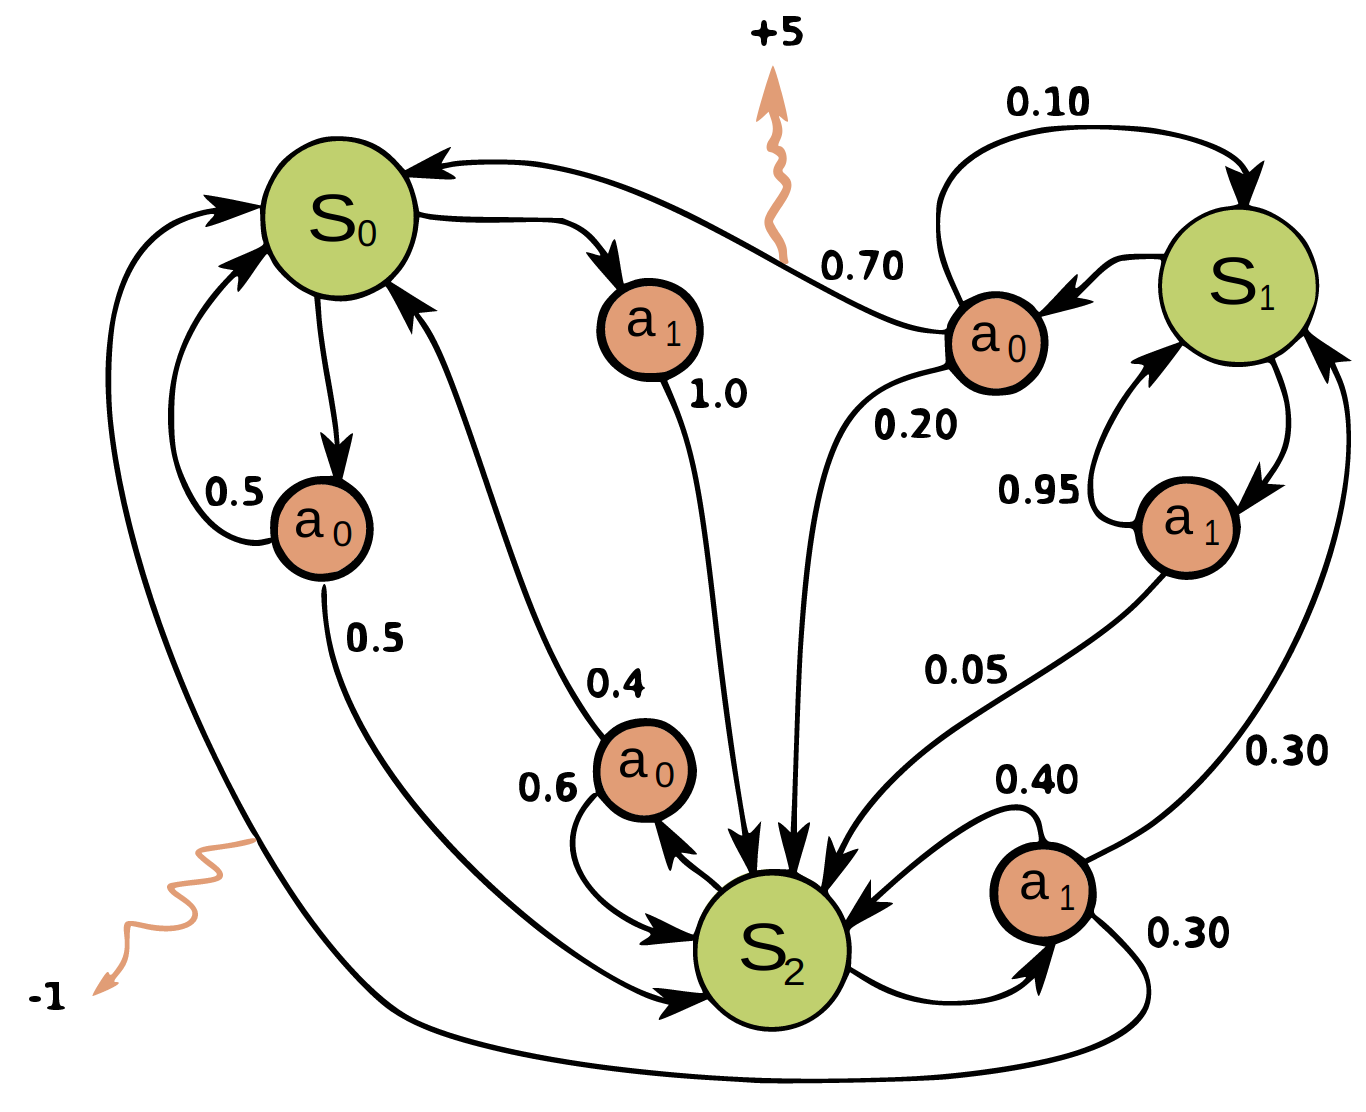
\includegraphics[height=1.8in]{figs/MDPwiki.png}
\caption{
Illustration of an MDP as a finite state machine (FSM).
The MDP has three discrete states (green cirlces),
two discrete
actions (orange circles), and two non-zero rewards (orange arrows).
The numbers on the black
edges represent state transition
probabilities, e.g.,  $p(s'=s_0|a=a_0,s'=s_0)=0.7$;
most state transitions are impossible
(probability 0), so the graph is sparse.
The numbers on the yellow wiggly edges represent
expected rewards, e.g., $R(s=s_1, a=a_0, s'=s_0) = +5$;
state transitions   with zero reward are not annotated.
\figtaken{\url{https://en.wikipedia.org/wiki/Markov_decision_process}}.
%\figtaken{\url{https://commons.wikimedia.org/wiki/File:Markov_Decision_Process.svg}}.
\figthanks{Wikipedia author waldoalvarez}.
}
\label{fig:MDP}
\end{figure}

A \keywordDef{Markov decision process}~\citep{Puterman94}
is a special case of a POMDP in which the environment states are observed,
so $z_t=o_t=s_t$.\footnote{
%
The field of \keyword{control theory}
uses slightly different terminology and notation.
In particular, 
the environment is called the \keywordDef{plant},
and the agent is called the \keywordDef{controller}.
States are denoted by $\vx_t \in \calX \subseteq \real^D$,
actions are denoted by $\vu_t \in \calU \subseteq \real^K$,
and rewards are replaced by costs $c_t \in \real$.
}
We usually define an MDP in terms of the state transition matrix
induced by the world model:
\be
\ptran(s_{t+1}|s_t,a_t) = \expectQ{\ind{s_{t+1}=W(s_t,a_t,\epsilon^s_t)}}{\epsilon^s_t}
\ee
In lieu of an observation model, we assume the environment
(as opposed to the agent) sends out a reward signal,
sampled from $p_R(r_t|s_t,a_t,s_{t+1})$.
The expected reward is then given by
\begin{align}
  R(s_t,a_t,s_{t+1}) &= \sum_r r  \;\; \preward(r|s_t,a_t,s_{t+1}) \\
  R(s_t,a_t) &= \sum_{s_{t+1}} \ptran(s_{t+1}|s_t,a_t) R(s_t,a_t,s_{t+1})
\end{align}
Given a stochastic policy $\pi(a_t|s_t)$,
the agent can interact with the environment over many steps.
Each step is called a \keywordDef{transition},
and consists of the tuple $(s_t,a_t,r_t,s_{t+1})$,
where $a_t\sim \policy(\cdot|s_t)$,
$s_{t+1} \sim \ptran(s_t,a_t)$,
and $r_t \sim \preward(s_t,a_t,s_{t+1})$.
Hence, under policy $\policy$,
the probability of generating a \keywordDef{trajectory}  length $T$,
$\traj=(s_0,a_0,r_0,s_1,a_1,r_1,s_2,\ldots, s_T)$,
can be written explicitly as
\begin{align}
\label{eqn:rl-traj-prob}
p(\traj) = \initdist(s_0) \prod_{t=0}^{T-1} \policy(a_t|s_t) \ptran(s_{t+1}|s_t,a_t)
\preward(r_t|s_t,a_t,s_{t+1})
\end{align}


In general, the state and action sets of an MDP can be discrete or continuous.
When both sets are finite,
we can represent these functions as lookup tables;
this is known as a \keywordDef{tabular representation}.
In this case, we can represent the MDP as a
\keywordDef{finite state machine},
which is a graph where nodes correspond to states,
and edges correspond to actions and the resulting rewards and next states.
\cref{fig:MDP} gives a simple example
of an MDP with 3 states and 2 actions.

If we know the world model $\ptran$ and $\preward$,
and if the state and action space is tabular,
then we can solve for the optimal policy
using dynamic programming techniques,
as we discuss in  \cref{sec:planning}.
However, typically the world model is unknown,
and the states and actions may need 
complex nonlinear models to represent their transitions.
In such cases, we will have to use RL methods to learn a good policy.






\subsection{Contextual MDPs}

A \keywordDef{Contextual MDP} \citep{Hallak2015}
is an MDP where the 
dynamics and rewards of the environment depend on a
hidden static parameter referred to as the context.
(This is different to a contextual bandit, discussed in \cref{sec:bandits},
where the context is observed at each step.)
A simple example of a contextual MDP is a
video game, where each level of the game
is \keywordDef{procedurally generated},
that is, it is randomly generated each time
the agent starts a new episode.
Thus the agent must solve a sequence of
related MDPs, which are drawn from a common distribution.
This requires the agent to \keywordDef{generalize} across multiple MDPs,
rather than overfitting to a specific environment
\citep{Cobbe2019,Kirk2021,Tomilin2022}.
(This form of generalization is different
from generalization within an MDP,
which requires generalizing across states,
rather than across environments; both are important.)

A contextual MDP is a special kind of POMDP
where the hidden variable corresponds to the unknown
parameters of the model.
In \citep{Ghosh2021RL}, they call this an \keywordDef{epistemic POMDP},
which is closely related to the concept
of belief state MDP which we discuss in \cref{sec:beliefStateMDP}.




\subsection{Contextual bandits}
\label{sec:contextualBandit}
\label{sec:bandits}

A \keywordDef{contextual bandit} is a special case of a POMDP
where the world state transition function is independent of the
action of the agent and the previous state,
i.e., $p(z_t|z_{t-1},a_t) = p(z_t)$.
In this case, we call the world states ``contexts'';
these are observable by the agent, i.e., $o_t=z_t$.
Since the world state distribution is independent of the agents actions,
the agent has no effect on the external
environment.
However, its actions do affect  the rewards that it
receives. Thus the agent's internal belief state --- about the underlying
reward function $R(o,a)$ --- does change over time,
as the agent learns a model of the world
(see \cref{sec:beliefStateMDP}).



A special case of a contextual bandit is a regular bandit,
in which there is no context, or equivalently, $s_t$ is
some fixed constant that never changes.
When there are a finite number of possible actions,
$\calA=\{a_1,\ldots,a_K\}$,
this is called a \keywordDef{multi-armed bandit}.\footnote{
%
The terminology arises by analogy to a slot machine
(sometimes called a ``bandit'')
in a casino.
If there are $K$ slot machines, each with different rewards
(payout rates), then the agent (player) must explore
the different machines until they have discovered
which one is best, and can then stick to exploiting it.
}
In this case the reward model  has the form $R(a) = f(\vw_a)$,
where $\vw_a$ are the parameters for arm $a$.



Contextual bandits have many applications.
For example, consider an \keywordDef{online advertising system}.
In this case, the state $s_t$ represents features
of the web page
that the user is currently looking at,
and the action $a_t$ represents the identity
of the  ad which the system
chooses to show.
Since the relevance of the ad depends on the page,
the reward function has the form $R(s_t,a_t)$,
and hence  the problem is contextual.
The goal is to maximize the expected reward,
which is equivalent to the expected number of times people click on
ads; this is known as
 the \keywordDef{click through rate} or \keywordDef{CTR}.
(See e.g.,  \citep{Graepel10,Li10linucb,McMahan13,Agarwal2014laser,Du2021ads,Yang2022CTR}
for more information about this application.)
Another application of contextual bandits
arises in \keywordDef{clinical trials}
\citep{Villar2015}.
In this case, the state $s_t$ are features of the current patient we are treating,
and the action $a_t$ is the treatment the doctor chooses to give them
(e.g., a new drug or a \keywordDef{placebo}).

%We discuss some ways of computing bandit policies with optimal regret
%in \cref{sec:explorationExploitation}.
For more details on bandits,
see e.g., \citep{Lattimore2019,Slivkins2019}.


\subsection{Belief state MDPs}
\label{sec:beliefStateMDP}

In this section, we describe a kind of MDP where the state
represents a probability distribution,
known as a \keywordDef{belief state} or \keywordDef{information state},
which is updated by the agent (``in its head'') as it receives
information from the environment.\footnote{
%
Technically speaking,  this is a POMDP, where we assume the states are observed,
and the parameters are the unknown hidden random variables.
This is in contrast to \cref{sec:POMDP},
where the states were not observed, and the parameters were assumed to be known.
} %
More precisely, consider a contextual bandit problem,
where the agent approximates the unknown reward by a function
$R(o,a)=f(o,a;\vw)$.
Let us denote the posterior over the unknown parameters
by $\bstate_t=p(\vw|\history_t)$,
where $\history_t = \{ o_{1:t}, a_{1:t}, r_{1:t} \}$
is the history of past observations, actions and rewards.
This belief state can be updated deterministically using Bayes' rule;
we denote this operation by
$\bstate_{t+1}=\mathrm{BayesRule}(\bstate_{t},o_{t+1},a_{t+1},r_{t+1})$.
(This corresponds to the state update $SU$ defined earlier.)
Using this, we can define the following
\keywordDef{belief state MDP},
with deterministic dynamics given by
\begin{align}
  p(\bstate_{t+1}|\bstate_{t},o_{t+1},a_{t+1},r_{t+1})
  &= \ind{\bstate_{t+1}=\mathrm{BayesRule}(\bstate_{t},o_{t+1},a_{t+1},r_{t+1})} 
\end{align}
and reward function given by
\begin{align}
p(r_t|o_t,a_t,\bstate_t) &= \int \preward(r_t|o_t,a_t;\vw) p(\vw|\bstate_t) d\vw
\end{align}
If we can solve this (PO)MDP, we have the optimal solution to the exploration-exploitation
problem. 

\begin{figure}
\centering
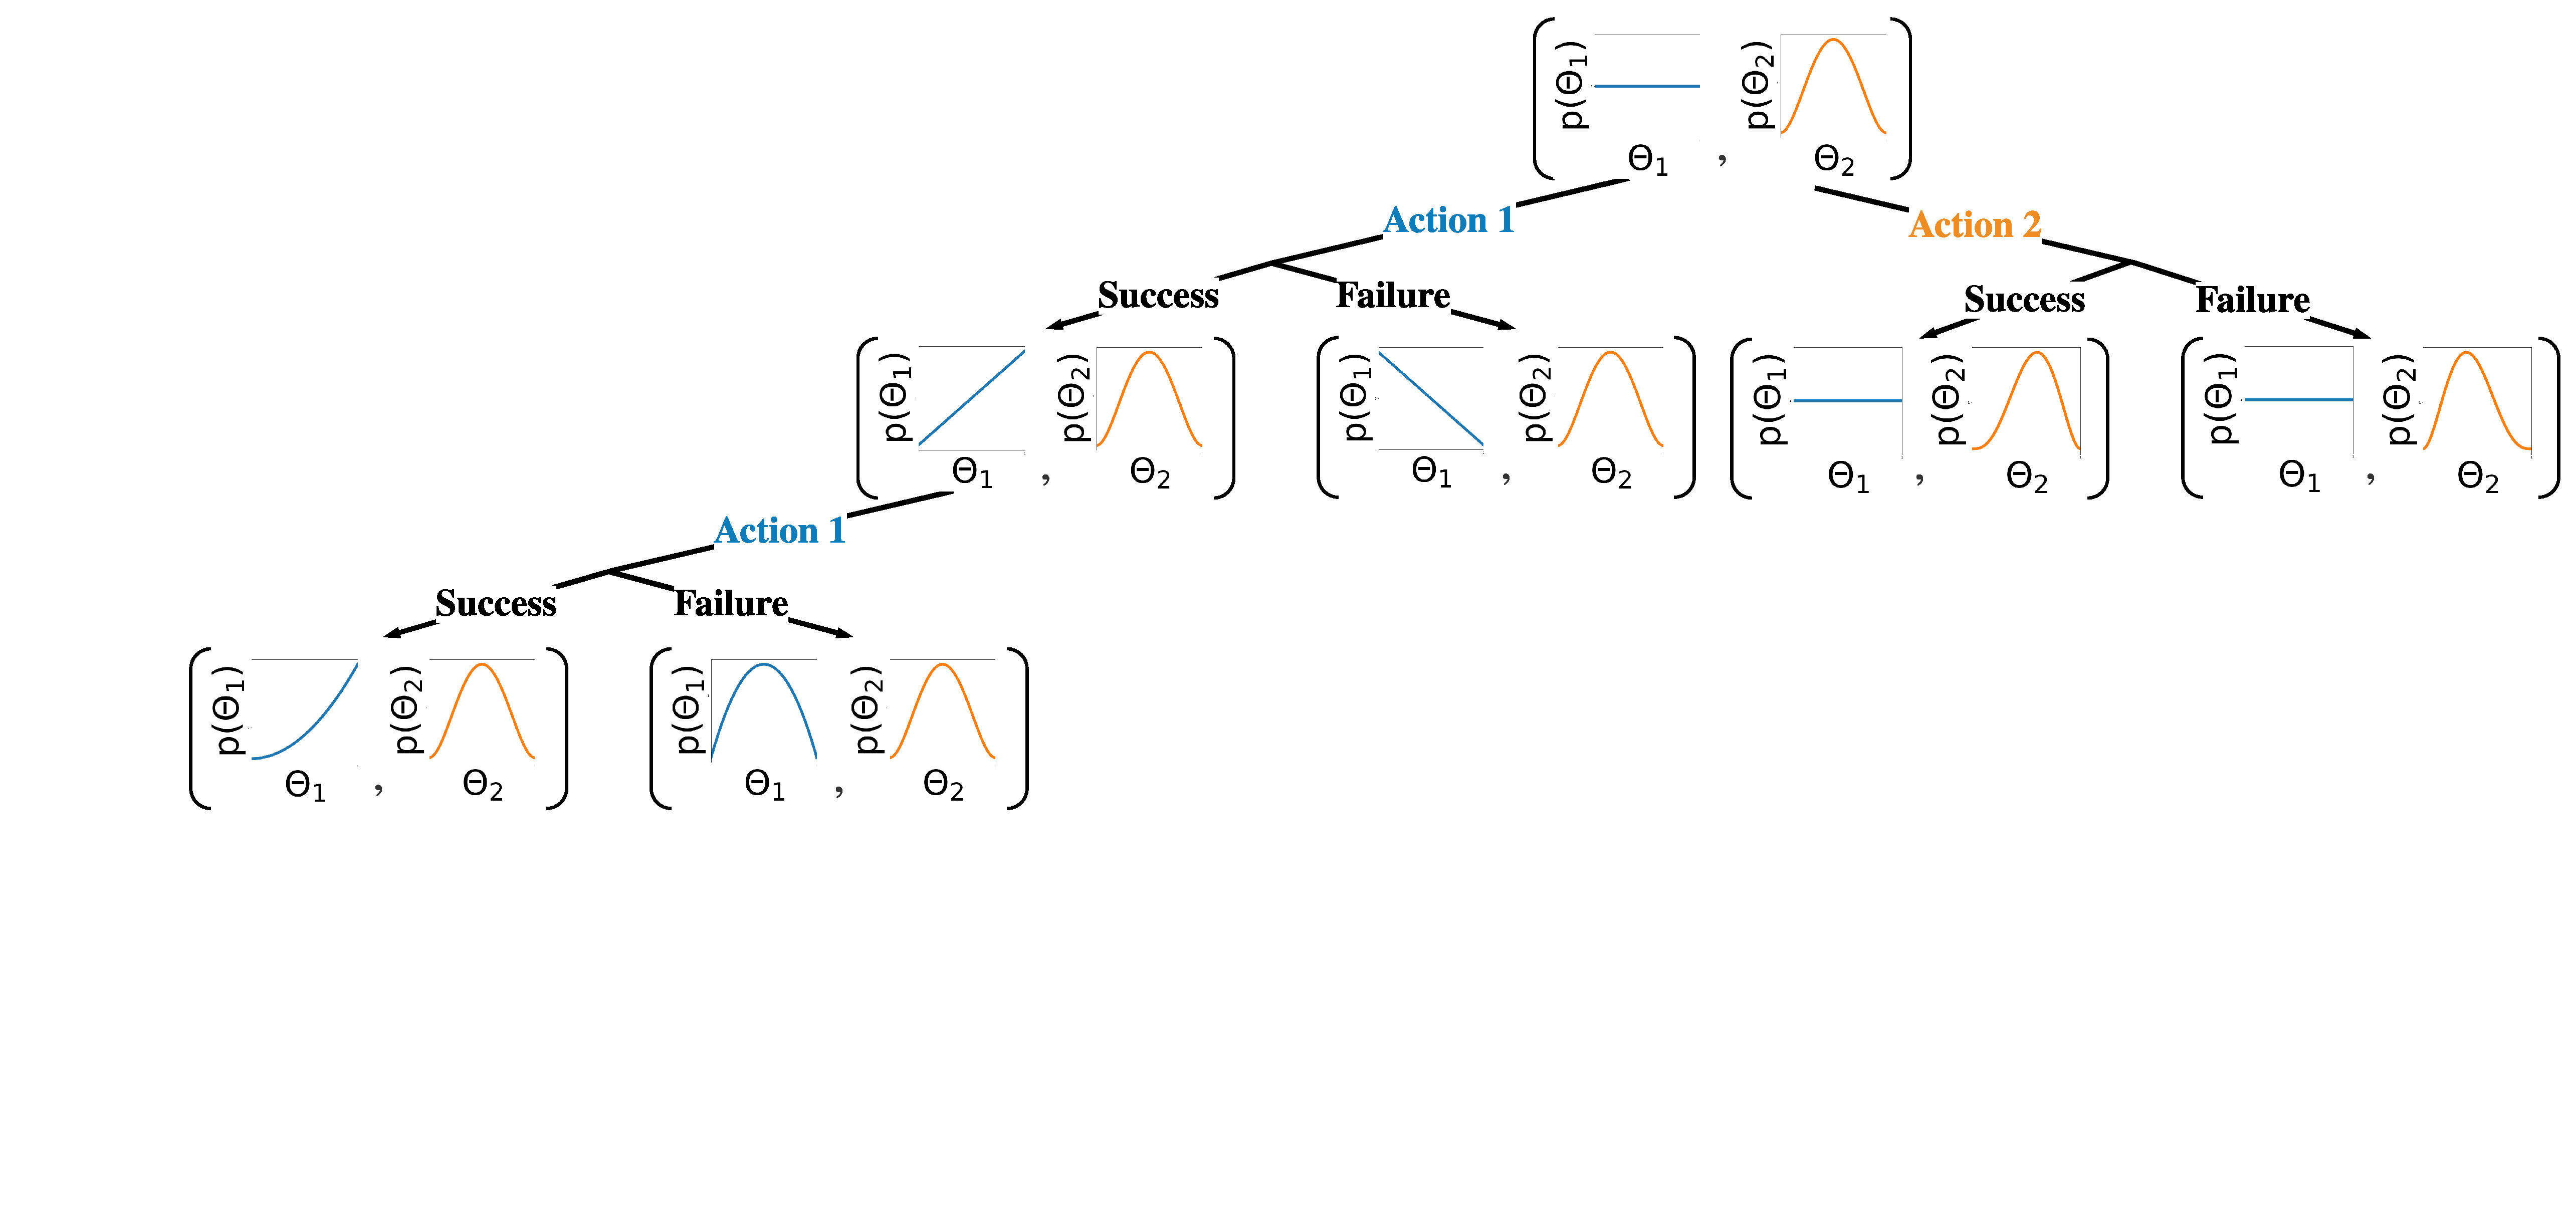
\includegraphics[height=2in]{figs/beta_bernoulli_bandit}
\caption{
Illustration of sequential belief updating
for a two-armed beta-Bernoulli bandit.
The prior for the reward for action 1
is the (blue) uniform distribution $\betadist(1,1)$;
the prior for the reward for action 2
is the (orange) unimodal distribution $\betadist(2,2)$.
We update the parameters of the belief state based on the chosen action,
and based on whether the observed reward is success (1)
or failure (0).
%where the arms correspond to different drugs in a clinical trial,
%and the observed outcomes (rewards)
%correspond to success or failure of the trial.
%(Compare to \cref{fig:sequentialCoinToss},
%where we display the predictive distribution
%for a single armed beta-Bernoull model.)
%  \figtaken{\citep{Silver2018L9}}.
%\figthanks{David Silver}.
%https://lucid.app/lucidchart/55b3264c-7ee4-42e5-a11d-74c6741c4b8b/edit?page=0_0&invitationId=inv_08240636-abf8-4d40-9db2-edd39d2b5e34#
%\figgen{\notebook{beta\_bernoulli\_bandits}}.
}
\label{fig:bernoulliBanditBAMDP}
\end{figure}


As a simple example,
consider 
a context-free \keywordDef{Bernoulli bandit},
where $\preward(r|a) = \Ber(r|\mu_a)$,
and $\mu_a=\preward(r=1|a)=R(a)$ is the expected reward for taking
action $a$.
The only unknown parameters are $\vw=\mu_{1:A}$.
Suppose  we use  a factored beta prior
\be
p_0(\vw)=\prod_a \betadist(\mu_a|\alpha_0^a,\beta_0^a)
\ee
where $\vw=(\mu_1,\ldots,\mu_K)$.
We can compute the posterior in closed form
to get
\be
p(\vw|\data_t) =
\prod_a \betadist(\mu_a|\underbrace{\alpha_0^a + N_{t}^0(a)}_{\alpha_t^a},
\underbrace{\beta_0^a + N_{t}^1(a)}_{\beta_t^a})
\label{eqn:postBetaBandit}
\ee
where
\be
N_t^r(a) = \sum_{i=1}^{t-1} \ind{a_i=a, r_i=r}
\ee
This is illustrated in \cref{fig:bernoulliBanditBAMDP}
for a two-armed Bernoulli bandit.
We can use a similar method for a \keywordDef{Gaussian bandit},
where $\preward(r|a)=\gauss(r|\mu_a,\sigma_a^2)$.

In the case of contextual bandits, the problem is conceptually
the same, but becomes more
complicated computationally.
If we assume a \keywordDef{linear regression bandit},
$\preward(r|s,a;\vw) = \gauss(r|\vfeatures(s,a)^\trans \vw,\sigma^2)$,
we can use Bayesian linear regression to compute
$p(\vw|\data_t)$ exactly in closed form.
If we assume a \keywordDef{logistic regression bandit},
$\preward(r|s,a;\vw) = \Ber(r|\sigmoid(\vfeatures(s,a)^\trans \vw))$,
we have to use approximate methods for approximate Bayesian logistic regression to compute
$p(\vw|\data_t)$.
If we have a \keywordDef{neural bandit}
of the form
$\preward(r|s,a;\vw) = \gauss(r|f(s,a; \vw))$
for some nonlinear function $f$,
then  posterior inference is even more challenging
(this is equivalent to the problem of inference
in Bayesian neural networks, see e.g., \citep{Arbel2023} for a review paper
for the offline case, and \citep{Duran-Martin2022,bong} for some recent online methods).

We can generalize the above methods to compute the belief state
for  the parameters of an MDP in the obvious way,
but modeling both the reward function and state transition function.


Once we have computed the belief state,
we can derive a policy with optimal  regret using the
methods  like UCB (\cref{sec:UCB})
or Thompson sampling (\cref{sec:thompson}).
%methods described in \cref{sec:explorationExploitation}.

\eat{
We can compute an optimal policy
for a contextual bandit by defining
the agent belief state  to be $s_t=\vb_t = p(\vw|\vh_t)$,
where $\vw$ are the weights of the reward model,
$R(o,a)=f(o,\vw)_a$ for some function $f$.
We can update this state using Bayes rule to give
$s_{t+1}=SU(s_t,a_t,r_{t+1})$.
The optimal policy $\pi(s_t)$ can be computed using the methods
described in
\cref{sec:beliefStateMDP},
although in practice is more common to use simpler heuristics
like UCB (\cref{sec:UCB})
or Thompson sampling (\cref{sec:thompson}).
}


\subsection{Optimization problems}
\label{sec:opt}

The  bandit problem is an example of a problem where the agent
must interact with the world in order to collect information,
but it does not otherwise affect the environment.
Thus the agents internal belief state changes over time,
but the environment state does not.\footnote{
%
In the contextual bandit problem, the environment state (context) does change,
but not in response to the agent's actions.
Thus $p(o_t)$ is usually assumed  to be a static distribution.
}
Such problems commomly arise when we are trying to optimize a fixed but unknown
function $R$. We can ``query'' the function by evaluating it at different
points (parameter values), and in some cases, the resulting observation
may also include gradient information.
The agent's goal is to find the optimum of the function in as few steps
as possible. We give some examples of this problem setting below.

\subsubsection{Best-arm identification}

In the standard multi-armed bandit problem
our goal is to maximize the sum of expected
rewards.
However, in some cases, the goal is to determine 
the best arm given a fixed budget of $T$ trials;
this variant is
known as \keywordDef{best-arm identification}~\citep{Audibert10Best}.
Formally, this corresponds to optimizing the \keywordDef{final reward}
criterion:
\be
V_{\pi,\pi_T} = \expectQ{R(\hat{a})}{p(a_{1:T}, r_{1:T}|s_0,\pi)}
\ee
where $\hat{a} = \pi_T(a_{1:T}, r_{1:T})$ is the estimated optimal arm
as computed by the \keywordDef{terminal policy} $\pi_T$
applied to the sequence of observations obtained by the exploration policy $\pi$.
This can be solved by a simple adaptation of the methods used for standard bandits.

\subsubsection{Bayesian optimization}
\label{sec:BO}

Bayesian optimization is a gradient-free approach to optimizing expensive blackbox functions.
That is, we want to find
\be
\vw^* = \argmax_{\vw} R(\vw)
\ee
for some unknown function $R$,
where $\vw \in \real^N$,
using as few actions (function evaluations of $R$) as possible.
This is essentially  an ``infinite arm'' version of the best-arm identification problem
\citep{Toussaint2014},
where we replace the discrete choice of arms $a \in \{1,\ldots,K\}$
with the parameter vector $\vw \in \real^N$.
In this case, the optimal policy can be computed
if the agent's state $s_t$ is a belief state over 
the unknown function, i.e., $s_t=p(R|\vh_t)$.
A common way to represent this distribution is to use Gaussian processes.
We can then use heuristics like expected improvement, knowledge gradient
or Thompson sampling
to implement the corresponding policy, $\vw_t=\pi(s_t)$.
For details, see e.g., \citep{Garnett2023}.

\subsubsection{Active learning}

Active learning is similar to BayesOpt, but instead of trying to find the point
at which the function is largest (i.e., $\vw^*$), we are trying to learn
the whole function $R$, again by querying it at different points $\vw_t$.
Once again, the optimal strategy again requires maintaining a belief state over the unknown function,
but now the best policy takes a different form, such as choosing query points
to reduce the entropy
of the belief state.
See e.g., \citep{Smith2023}.


\subsubsection{Stochastic Gradient Descent (SGD)}

Finally we discuss how to interpret SGD as a sequential decision making process,
following \citep{Powell2022}.
The action space  consists of querying the unknown function $R$ at
locations $\va_t=\vw_t$, and observing the function value $r_t=R(\vw_t)$;
however, unlike BayesOpt, now we also observe
the corresponding gradient $\vg_t = \nabla_{\vw} R(\vw)|_{\vw_t}$,
which gives non-local information about the function.
The environment state contains the true function $R$
which is used to generate the observations given the agent's actions.
The agent state contains the current parameter estimate
$\vw_t$, and may contain  other information such as first and second moments
$\vm_t$ and $\vv_t$,
needed by methods such as Adam.
The update rule (for vanilla SGD) takes the form
$\vw_{t+1}=\vw_t + \alpha_t \vg_t$,
where the stepsize $\alpha_t$ is chosen by the policy,
$\alpha_t=\pi(s_t)$.
The terminal policy has the form $\pi(s_T)=\vw_T$.

Although in principle it is possible to learn the learning rate (stepsize) policy
using RL (see e.g., \citep{Xu2017RL}), the policy is usually
chosen by hand, either using a \keywordDef{learning rate schedule}
or some kind of manually designed \keywordDef{adaptive learning rate} policy
(e.g., based on second order curvature information).




\section{Reinforcement Learning}
\label{sec:RLoverview}


In this section, we give a
brief overview of how to compute
optimal policies when the model of the environment is unknown;
this is the core problem tackled by RL.
We mostly  focus on the MDP case, but discuss the POMDP case
in \cref{sec:partialObs}.

We may categorize RL methods along two main
dimensions:
(1) by what
the agent represents and learns:
the value function,
and/or the policy,
and/or the model;
(2) and by how actions are selected:
\keywordDef{on-policy} (actions must be selected by the agent's
current policy),
and \keywordDef{off-policy}
(actions can be select by any kind of policy,
including human demonstrations).
\cref{tab:RL} lists a few representative examples.
More details are given in the subsequent sections.


\begin{table}
  \centering
\begin{tabular}{lllll}
Approach &  Method & Functions learned & On/Off & Section
  \\ \hline
Value-based &  SARSA & $Q(s,a)$ & On & \cref{sec:SARSA} \\          
Value-based &   $Q$-learning & $Q(s,a)$ & Off & \cref{sec:Qlearning} 
  \\ \hline
Policy-based &  REINFORCE & $\policy(a|s)$ & On & \cref{sec:REINFORCE} \\
Policy-based &   A2C & $\policy(a|s)$, $V(s)$ & On &  \cref{sec:A2C} \\      
Policy-based &   TRPO/PPO & $\policy(a|s)$, $\advantage(s,a)$ & On & \cref{sec:PPO} \\
Policy-based &   DDPG & $a=\policy(s)$, $Q(s,a)$ & Off & \cref{sec:DDPG} \\
Policy-based &   Soft actor-critic & $\policy(a|s)$, $Q(s,a)$ & Off & \cref{sec:SAC} 
  \\ \hline
Model-based &  MBRL & $p(s'|s,a)$ & Off & \cref{sec:MBRL}
\end{tabular}
\caption{
  Summary of some popular methods for RL.
  On/off refers to on-policy vs off-policy methods.
}
\label{tab:RL}
\end{table}


\subsection{Value-based RL (Approximate Dynamic Programming)}
\label{sec:rl-intro-valuebased}

In this section, we give a brief introduction to \keywordDef{value-based RL},
also called \keywordDef{Approximate Dynamic Programming} or \keywordDef{ADP};
see \cref{sec:valueRL} for more details.

We introduced the value function $\Vpol(s)$ in \cref{eqn:valueFn},
which we repeat here for convenience:
\begin{align}
\Vpol(s)
\defeq \expectQ{\return_0 | s_0=s}{\policy}
=\expectQ{\sum_{t=0}^{\infty} \gamma^t r_{t} | s_0=s}{\policy}
\end{align}
The value function for the optimal policy $\pi^*$
is known to satisfy the following recursive condition,
known as 
\keywordDef{Bellman's equation}:
\begin{align}
  \Vopt(s) &=
   \max_a R(s,a) + \gamma \expectQ{\Vopt(s')}{\ptran(s'|s,a)} 
\end{align}
This follows from the principle of \keywordDef{dynamic programming},
which computes the optimal solution to a problem (here the value of state $s$
by combining
the optimal solution of various subproblems (here the values
of the next states $s'$).
This can be used to derive the following learning rule:
\be
V(s) \leftarrow V(s) + \lr[r + \gamma V(s') - V(s)]
\ee
where $s' \sim \ptran(\cdot|s,a)$
is the next state sampled from the environment,
and $r=R(s,a)$ is the observed reward.
This is called  \keywordDef{Temporal Difference} or \keywordDef{TD} learning
(see \cref{sec:TD} for details).
Unfortunately,  it is not clear how to derive a policy if all we know is the
value function.
We now describe a solution to this problem.

We first generalize the notion of value function
to assigning a value to a state and action pair, by defining the
\keywordDef{Q function} as follows:
\begin{align}
\Qpol(s,a)
\defeq \expectQ{\return_0 | s_0=s,a_0=a}{\policy}
=\expectQ{\sum_{t=0}^{\infty} \gamma^t r_{t} | s_0=s,a_0=a}{\policy}
\end{align}
This quantity represents the expected return obtained
if we start by taking action $a$ in state $s$,
and then follow $\policy$ to choose actions thereafter.
The $Q$ function for the optimal policy
satisfies a modified Bellman equation
\begin{align}
    \Qopt(s,a) &= R(s,a) + \gamma  \expectQ{\max_{a'} \Qopt(s',a')}{\ptran(s'|s,a)}
\end{align}
This gives rise to the following TD update rule:
\begin{align}
  Q(s,a) \leftarrow
r + \gamma \max_{a'} Q(s',a')- Q(s,a)
\end{align}
where we sample $s' \sim \ptran(\cdot|s,a)$ from the environment.
The action is chosen at each step from the implicit policy
\be
a = \argmax_{a'} Q(s,a')
\ee
This is called \keywordDef{Q learning}
(see \cref{sec:Qlearning} for details),

\eat{
we try to learn the optimal $Q$-function from experience,
and then derive a policy from it using \cref{eqn:optPolFromQ}.
Typically, a function approximator
(e.g., a neural network), $\Qapprox$,
is used to represent the $Q$-function,
which is trained iteratively.
Given a transition $(s,a,r,s')$, we define
the \keywordDef{temporal difference}
(also called the \keywordDef{TD error}) as
\begin{align}
r + \gamma \max_{a'} \Qapprox(s',a')- \Qapprox(s,a)
\end{align}
Clearly, the expected TD error is the Bellman error evaluated at $(s,a)$.
Therefore, if $\Qapprox=\Qopt$, the TD error is $0$ on average by Bellman's optimality equation.
Otherwise, the error provides a signal
for the agent to change $\vw$ to make
$\Qapprox(s,a)$ closer to $R(s,a) + \gamma \max_{a'} \Qapprox(s',a')$.
The update on $\Qapprox$ is based on a target
that is computed using $\Qapprox$.
This is called \keywordDef{Q-learning}.
This kind of update is known as \keywordDef{bootstrapping} in RL,
and should not be confused with the
statistical bootstrap.
Value based methods are discussed in more detail in \cref{sec:RLvalue}.
}

\subsection{Policy-based RL}

In this section we give a brief introductin
to \keywordDef{Policy-based RL}; for details see  \cref{sec:policySearch}.

In policy-based methods,
we try to directly maximize $J(\pi_{\vtheta})=\expectQ{V_{\pi}(s_0)}{p(s_0)}$
wrt the parameter's $\vtheta$;
this is called \keywordDef{policy search}.
If $\polval(\polapprox)$ is differentiable wrt $\vtheta$,
we can use stochastic gradient ascent to optimize
$\vtheta$, which is known as
\keywordDef{policy gradient} (see \cref{sec:PG}).

Policy gradient methods have the advantage that
they provably converge to a local optimum
for many common policy classes,
whereas $Q$-learning may diverge
when approximation is used
(\cref{sec:offpolicyrl-deadlytriad}).
In addition, policy gradient methods can easily be applied to
continuous action spaces, 
since they do not need to compute $\argmax_a Q(s,a)$.
Unfortunately,
the score function estimator
for $\nabla_{\vtheta} \polval(\polapprox)$ can have a very high 
variance, so the resulting method can converge slowly.

One way to reduce the variance is to learn
an approximate value function, $\Vapprox(s)$,
and to use it as a baseline
in the score function estimator.
We can learn $\Vapprox(s)$ using 
using TD learning.
Alternatively, we can learn an advantage function,
$\Aapprox(s,a)$, and use it as a baseline.
These policy gradient variants are called
\keywordDef{actor critic} methods,
where the actor refers to the policy $\polapprox$
and the critic refers to $\Vapprox$ or $\Aapprox$.
See \cref{sec:AC} for details.



\subsection{Model-based RL}

In this section, we give a brief introduction to \keywordDef{model-based RL};
for more details, see
\cref{sec:MBRL}.

Value-based methods, such as Q-learning,
and policy search methods, such as policy gradient,
can be very \keywordDef{sample inefficient},
which means they may need to interact with the environment many times
before finding a good policy,
which can be problematic when real-world interactions are expensive.
In \keyword{model-based RL},
we first learn the MDP,
including  the $\ptran(s'|s,a)$ and $R(s,a)$ functions,
and then compute the policy, either using approximate dynamic programming
on the learned model, or doing lookahead search.
In practice, we often interleave the model learning
and planning phases,
so we can use the partially learned policy to decide
what data to collect, to help learn a better model.

\subsection{Dealing with partial observability}
\label{sec:partialObs}

In an MDP, we assume that the state of the environment $s_t$
is the same as the observation $o_t$ obtained by the agent.
But in many problems, the observation only gives partial information
about the underlying state of the world
(e.g., a rodent or robot navigating in a maze).
This is called \keywordDef{partial observability}.
In this case, using a policy of the form
$a_t = \pi(o_t)$ is suboptimal, since $o_t$
does not give us complete state information.
Instead we need to use a policy of the form
$a_t = \pi(\vh_t)$,
where $\vh_t=(a_1, o_1,  \ldots, a_{t-1}, o_t)$
is the entire past history of observations and actions,
plus the current observation.
Since depending on the entire past is not tractable
for a long-lived agent, various approximate solution methods
have been developed, as we summarize below.

\subsubsection{Optimal solution}

If we know the true latent structure of the world
(i.e., both $p(o|z)$ and $p(z'|z,a)$, to use the notation
of \cref{sec:universal}),
then we can use solution methods designed
for  \keyword{POMDPs}, discussed in \cref{sec:POMDP}.
This requires using Bayesian inference to  compute a belief state,
$\vb_t = p(\vz_t|\vh_t)$ (see \cref{sec:beliefStateMDP}),
and then using this belief state
to guide our decisions.
\eat{
In particular, we can derive the corresponding
\keywordDef{belief state MDP},
in which the states are belief states,
and the state dynamics are deterministic (conditional on the next
observation), as given by Bayes' rule:
\be
p(\vb_{t+1}|\vb_t,\vo_{t+1},\va_t)
\propto p(\vb_{t+1}|\vb_t, \va_t) p(\vo_{t+1}|\vb_{t_1})
\ee
}
However, learning the parameters of a POMDP (i.e., 
the  generative latent world model) is very difficult,
as is recursively computing and updating the belief state,
as is computing the policy given the belief state.
Indeed, optimally solving POMDPs is known to be
computationally very difficult for any method
\citep{Papadimitriou87,Kaelbling98}.
So in practice simpler approximations are used.
We discuss some of these below.
(For more details, see \citep{Murphy00pomdp}.)

Note that it is possible to 
marginalize out the POMDP
latent state $z_t$,
to derive a prediction over the next observable state,
$p(\vo_{t+1}|\vh_t,\va_t)$.
This can then become a learning  target for a model, that is trained
to directly
predict  future observations, without explicitly invoking the concept
of latent state.
This is called a \keywordDef{predictive state representation}
or \keywordDef{PSR} \citep{PSR}.
This is related to the idea of
\keywordDef{observable operator models}
\citep{Jaeger2000},
and to the concept of
successor representations
which we discuss in  \cref{sec:SR}.


\subsubsection{Finite observation history}

The simplest solution to the partial
observability problem is to  define
the state to be a finite history of the last $k$ observations,
$\vs_t = \vh_{t-k:t}$;
when the observations $\vo_t$ are images,
this is often called \keywordDef{frame stacking}.
We can then use standard MDP methods.
Unfortunately, this cannot capture long-range dependencies in the data.

\subsubsection{Stateful (recurrent) policies}
  
A more powerful approach is to use a stateful policy,
that can remember the entire past, and not just respond
to the current input or last $k$ frames.
For example, we can represent the policy by an RNN (recurrent neural
network),
 as proposed in  the \keywordDef{R2D2} paper \citep{R2D2},
 and used in many other papers.
Now the hidden state $\vz_t$ of the RNN
will implicitly summarize the past observations, $\vh_t$,
and can be used in lieu of the state $s_t$ in any standard RL algorithm.


RNNs policies are widely used, and this method is often effective in solving partially
observed problems. However, they typically will not plan to perform
information-gathering actions, since there is no explicit notion of
belief state or uncertainty. However, such behavior can arise
via meta-learning \citep{Mikulik2020}.

\eat{
Alternatively, \citep{Moss2024} present an approach
called \keywordDef{BetaZero}, that amortizes look ahead search
in belief space into a neural network,
analogous to MuZero (\cref{sec:muzero}).
Since this plans in the space of distributions,
it can choose to perform information gathering actions.
}



\subsection{Software}

Implementing RL algorithms is much trickier than
methods for supervised learning,
or generative  methods such as language modeling
and diffusion,
all of which have stable (easy-to-optimize) loss functions.
Therefore it is often wise to build on existing
software rather than starting from scratch.
We list  some useful 
libraries  in \cref{tab:software}.

In addition, RL experiments can be very high variance,
making it hard to draw valid conclusions.
See \citep{Agarwal2021RL,Patterson2024,Jordan2024} for some recommended
experimental practices.
For example, when reporting performance across different environments,
with different intrinsic difficulties (e.g., different kinds
of Atari games),
\citep{Agarwal2021RL} recommend
reporting the \keywordDef{interquartile mean} (IQM) of the performance metric,
which is the mean of the samples between the 0.25 and 0.75 percentiles,
(this is a special case of a trimmed mean).
Let this estimate be denoted by $\hat{\mu}(\data_i)$,
where $\data$ is the empirical data (e.g., reward vs time)
from the $i$'th run.
We can estimate the uncertainty in this estimate using
a nonparametric method, such as bootstrap resampling,
or a parametric approximation, such as
a Gaussian approximation. (This requires computing
the standard error of the mean, $\frac{\hat{\sigma}}{\sqrt{n}}$,
where $n$ is the number of trials,
and $\hat{\sigma}$ is the estimated  standard deviation
of the (trimmed) data.)


\begin{table}
%  \begin{sidewaystable}
  \centering
  \footnotesize
  \begin{tabular}{lll}
    URL & Language & Comments \\ \hline
%    & Value algos & Policy algos & Model algos \\ \hline
    \href{https://github.com/EdanToledo/Stoix}{Stoix}
    & Jax & Mini-library with many methods (including MBRL)
%   & (Double) DQN, Dueling DQN, C51, Munchausen DQN,    QR-DQN,   Rainbow,
    %  &  Reinforce, DDPG, TD3, SAC,    PPO, DPO, MPO, VMPO, AWR,
%  &  AlphaZero, (Sampled) MuZero
    \\
    \href{https://github.com/luchris429/purejaxrl/tree/main}{PureJaxRL}
    & Jax & Single files with DQN; PPO, DPO
    \\
    \href{https://github.com/ikostrikov/jaxrl}{JaxRL}
    & Jax & Single files  with AWAC, DDPG, SAC, SAC+REDQ
        \\
    \href{https://stable-baselines3.readthedocs.io/en/master/guide/sbx.html}
         {Stable Baselines Jax}
         & Jax & Library with  DQN, CrossQ, TQC;  PPO, DDPG, TD3, SAC
%         & DQN, CrossQ, TQC
%         & PPO, DDPG, TD3, SAC
%         & None
     \\
     \href{https://github.com/tinker495/jax-baseline}{Jax Baselines}
     &  Jax & Library with many methods
     %& DQN, C51, QR-DQN, IQN, FQF, SPR, BBF
     %& A2C, PPO, TPPO, DDPG, TD3, TD7, SAC, TQC,
     %     & None
     \\
     \href{https://github.com/keraJLi/rejax}{Rejax}
     & Jax & Library with DDQN, PPO, (discrete) SAC, DDPG
     \\
         \href{https://github.com/google/dopamine}{Dopamine}
%         & Jax/TF & Library with DQN, QR-DQN, DrQ, DER, C51, Rainbow, IQN, SPR; SAC, PPO
         & Jax/TF & Library with many methods
\\
     \href{https://github.com/google-deepmind/rlax/tree/master}{Rlax}
     & Jax & Library of RL utility functions (used by Acme)
     \\
     \href{https://github.com/google-deepmind/acme/tree/master}{Acme}
     & Jax/TF & Library with many methods (uses rlax)
     \\
         \href{https://github.com/vwxyzjn/cleanrl}{CleanRL}
    & PyTorch & Single files with many methods
%    & DQN, C51, Qdagger,
%    & PPO, SAC, DDPG, TD3, PPG, RND
%    & None
    \\
    \href{https://stable-baselines3.readthedocs.io/en/master/}{Stable
      Baselines 3}
    & PyTorch & Library with DQN; A2C, PPO, DDPG, TD3, SAC, HER
%    & DQN
%    & A2C, PPO, DDPG, TD3, SAC, HER
    %    & None
    \\
    \href{https://github.com/thu-ml/tianshou/}{TianShou}
    & PyTorch & Library with many methods (including offline RL)
    \end{tabular}
  \label{tab:software}
  \caption{Some open source RL software.}
\end{table}
%\end{sidewaystable}

% https://github.com/tinker495/jax-baseline has Munchausen, High-Low
% Gauss, BBF, etc

% https://github.com/google-deepmind/dqn_zoo/

\eat{

  Google code
  
  We may be about to open pandora's box of online RL methods. There are several external JAX implementations such as PureJaxRL  (environment and agent both in JAX) and Gymnax (only agent is in JAX, IIUC). 
For the record, I am also  copying a list from Pablo about internal codebases:
-Xebulba is a very good starting point (and initial experiments have already been conducted there), as it supports distributed training and already includes implementations of many algorithms.
-Reverb is a general-purpose storage system, typically used as a replay buffer for distributed RL training. It’s distributed design is different from that of Xebulba, so using both may provide us with a diverse set of viewpoints/insights into this problem.
-Dopamine is another option, in particular for synchronous training. We have recently added a new replay buffer which will allow us to integrate with Reverb, thus enabling distributed training.
-RLX is used for fine-tuning LLMs with RLHF, and supports both
synchronous and distributed actors and learners
}


\section{Exploration-exploitation tradeoff}
\label{sec:exploreExploit}
\label{sec:explorationExploitation}
\label{sec:explore-exploit}

A fundamental problem in RL with unknown 
transition and reward models
is to decide between choosing
actions that the agent knows will yield high reward,
or choosing actions whose reward is uncertain,
but which may yield information
that helps the agent get to parts of state-action space
with even higher reward.
This is called the 
\keywordDef{exploration-exploitation tradeoff}.
In this section, we discuss various solutions.

%simple uniformed or undirected
%heuristics for solving the explore-exploit dilemma.
%We discuss more principled solutions in
%\cref{sec:exploreExploitRevisited}.

\subsection{Simple heuristics}
\label{sec:epsGreedy}

We start with a policy based on pure exploitation.
This is known as the 
\keywordDef{greedy policy},
$a_t=\argmax_a Q(s,a)$.
We can add exploration to this by 
sometimes picking some other, non-greedy action.

One approach
is to use an
\keywordSpecial{$\epsilon$-greedy}{epsilon-greedy} policy
$\policy_\epsilon$, parameterized by $\epsilon\in[0,1]$. 
In this case,  we pick
the greedy action wrt the current model,
$a_t = \argmax_a \estR_t(s_t,a)$ with probability
$1-\epsilon$, and a random action with probability $\epsilon$.
This rule ensures the agent's continual exploration
of all state-action combinations.
Unfortunately, this heuristic can be shown to be suboptimal,
since it explores every action with at least a constant
probability $\epsilon/|\calA|$,
although this can be solved by annealing $\epsilon$ to 0 over time.


Another problem with $\epsilon$-greedy is that it can result in ``dithering'',
in which the agent continually changes its mind about what to do.
In \citep{Dabney2021} they propose a simple solution to this
problem, known as
\keywordSpecial{$\epsilon z$-greedy}{epsilon-z-greedy},
that often works well.
The idea  is that with probability $1-\epsilon$ the agent
exploits, but with with probability $\epsilon$ the agent
explores by repeating the sampled action for $n \sim z()$ steps
in a row, where $z(n)$ is a distribution over the repeat duration.
This can help the agent escape from local minima.





\label{sec:boltzmannExploration}
Another approach is to use 
\keywordDef{Boltzmann exploration},
which assigns higher probabilities to explore more promising actions,
taking itno account the reward function.
That is, we use a polocy of the form
\be
\policy_{\tau}(a|s) = \frac{\exp(\estR_t(s_t,a)/\tau)}{\sum_{a'} \exp(\estR_t(s_t,a')/\tau)}
\ee
where $\tau>0$ is a temperature parameter
that controls how entropic the distribution is.
As $\tau$ gets close to $0$, $\policy_{\tau}$ becomes close to a greedy policy.  
On the other hand, higher values of $\tau$ will make
$\policy(a|s)$ more uniform, and encourage more exploration.
Its action selection probabilities can be much ``smoother'' with
respect to changes in the reward estimates 
than $\epsilon$-greedy, as illustrated in
\cref{tab:epsGreedy}.

\begin{table}
  \centering
\begin{tabular}{llllll}
  $\estR(s,a_1)$ & $\estR(s,a_2)$
  & $\policy_{\epsilon}(a|s_1)$     & $\policy_{\epsilon}(a|s_2)$  
    & $\policy_{\tau}(a|s_1)$     & $\policy_{\tau}(a|s_2)$     \\
  \hline
  1.00 & 9.00 & 0.05 & 0.95 & 0.00 & 1.00 \\
  4.00 & 6.00 & 0.05 & 0.95 & 0.12 & 0.88 \\
  4.90 & 5.10 & 0.05 & 0.95 & 0.45 & 0.55 \\
  5.05 & 4.95 & 0.95 & 0.05 & 0.53 & 0.48 \\
  7.00 & 3.00 & 0.95 & 0.05 & 0.98 & 0.02 \\
  8.00 & 2.00 & 0.95 & 0.05 & 1.00 & 0.00
\end{tabular}
\caption{Comparison of $\epsilon$-greedy policy (with $\epsilon=0.1$)
  and Boltzmann policy (with $\tau=1$) for a simple MDP with 6
  states and 2 actions.
  \figbased{Table 4.1 of \citep{Graesser2019}}.
  % p87
}
  \label{tab:epsGreedy}
\end{table}


The Boltzmann policy explores equally widely in all states.
An alternative approach is to try to explore (state,action)
combinations where the consequences of the outcome
might be uncertain.
This can be achived using  an \keywordDef{exploration bonus}
$R^b_t(s,a)$, which is large if the number
of times we have tried actioon $a$ in state $s$ is small.
We can then add $R^b$ to the regular reward,
to bias the behavior in a way that will hopefully
cause the agent to learn useful information
about the  world.
This is called an \keywordDef{intrinsic reward} function
(\cref{sec:intrinsicReward}).



\subsection{Methods based on the belief state MDP}


We can compute an optimal solution to the exploration-exploitation
tradeoff by adopting a Bayesian approach to the problem.
We start by computing the belief state MDP, as discussed in
\cref{sec:beliefStateMDP}.
We then compute the optimal policy, as we explain below.



\subsubsection{Bandit case (Gittins indices)}
\label{sec:gittins}


Suppose we have a way to compute the recursively compute
the belief state over model parameters,
$p(\vtheta_t|\data_{1:t})$.
How do we use this to solve for the policy
in the resulting belief state MDP?

In the special case of context-free bandits with a finite number of arms,
the optimal policy of this belief state MDP can be computed
using dynamic programming.
The result can be represented as a table of action probabilities,
$\pi_t(a_1,\ldots,a_K)$,
for each step;
this are known as  \keywordDef{Gittins indices}
\citep{Gittins89}
(see \citep{Powell2012,Powell2022} for a detailed explanation).
However, computing the optimal policy
for general  contextual bandits is intractable
\citep{Papadimitriou87}.

\subsubsection{MDP case (Bayes Adaptive MDPs)}
\label{sec:BAMDP}

We can extend the above techniques to the MDP case
by constructing a \keywordDef{BAMDP},
which stands for ``Bayes-Adaptive MDP''
\citep{Duff02}.
However, this is computationally intractable to solve,
so various approximations are made
(see e.g., \citep{Zintgraf2021,Arumugam2022bamdp,Mikulik2020}).
%borrowing from the \keywordDef{Bayesian RL} literature.
%See e.g., \citep{Ghavamzadeh2015} for details.


\subsection{Upper confidence bounds (UCBs)}
\label{sec:UCB}

The optimal solution to explore-exploit is intractable.
However, an intuitively sensible approach
is based on the principle known as
``\keywordDef{optimism in   the face of uncertainty}''
(OFU).
The principle selects actions greedily, but based on
optimistic estimates of their rewards.
The optimality of this approach is proved in the
\keywordDef{R-Max} paper of \citep{Tennenholtz2002},
which builds on the earlier \keywordDef{E3} paper of
\citep{Kearns2002}.

The most common implementation of this principle is
based on the notion of an
\keywordDef{upper confidence bound} or \keywordDef{UCB}.
We will initially explain this for the bandit case, then extend to the MDP case.

\subsubsection{Basic idea}

To use a UCB strategy, the agent maintains an optimistic reward
function estimate $\optR_t$, so that $\optR_t(s_t,a) \ge R(s_t,a)$ for
all $a$ with high probability, and then chooses the greedy action
accordingly: 
\begin{align}
a_t = \argmax_a \optR_t(s_t,a)
\end{align}
UCB can be viewed a form of \keywordDef{exploration bonus}, where the optimistic
estimate encourages exploration.  Typically, the amount of optimism,
$\optR_t - R$, decreases over time so that the agent gradually reduces
exploration.  With properly constructed optimistic reward estimates,
the UCB strategy has been shown to achieve near-optimal regret in many
variants of bandits~\citep{Lattimore2019}.
(We discuss regret in \cref{sec:regret}.)

The optimistic function $\optR$ can be obtained in different ways,
sometimes in closed forms, as we discuss below.

\subsubsection{Bandit case: Frequentist approach}

A frequentist approach to computing a confidence bound
can be based on a
\keywordDef{concentration inequality}~\citep{Boucheron16} to derive a
high-probability upper bound of the estimation error: $|\estR_t(s,a) -
R_t(s,a)| \le \delta_t(s,a)$, where $\estR_t$ is a usual estimate of
$R$ (often the MLE), and $\delta_t$ is a properly selected function.
An optimistic reward is then obtained by setting 
$\optR_t(s,a) = \estR_t(s,a) + \delta_t(s,a)$.

As an example, consider again the context-free Bernoulli bandit,
$R(a) \sim \Ber(\mu(a))$.
The  MLE $\estR_t(a)=\hat{\mu}_t(a)$ is given by
the empirical average of observed rewards whenever action $a$ was taken:
\begin{align}
  \hat{\mu}_t(a) &= \frac{N_t^1(a)}{N_t(a)} = \frac{N_t^1(a)}{N_t^0(a) + N_t^1(a)}
  \label{eqn:dtheory-bandit-mlebernoulli} 
\end{align}
where $N_t^r(a)$ is the number of times (up to step $t-1$)
that action $a$ has been tried
and the observed reward was $r$,
and $N_t(a)$ is the total number of times action $a$ has been tried:
\be
N_t(a) = \sum_{s=1}^{t-1} \ind{a_t=a}
\ee
Then the \keywordDef{Chernoff-Hoeffding inequality}
\citep{Boucheron16} leads to
$\delta_t(a) = c / \sqrt{N_t(a)}$
for some constant $c$, so
\begin{align}
  \optR_t(a) = \hat{\mu}_t(a) + \frac{c}{\sqrt{N_t(a)}}
  \label{eqn:UCBchernoff}
\end{align}

\subsubsection{Bandit case: Bayesian approach}

We can also derive an upper confidence about using  Bayesian inference.
If we use a beta prior, we can compute the posterior in closed form,
as shown in \cref{eqn:postBetaBandit}.
The posterior mean is
$\hat{\mu}_t(a) = \expect{\mu(a)|\history_t}=\frac{\alpha_t^a}{\alpha_t^a+\beta_t^a}$,
and 
the posterior standard deviation is approximately
\be
\hat{\sigma}_t(a) = \sqrt{\var{\mu(a)|\history_t}}
\approx \sqrt{\frac{\hat{\mu}_t(a) (1-\hat{\mu}_t(a))}{N_t(a)}}
\ee

We can use similar techniques for a
\keyword{Gaussian bandit},
where
$\preward(R|a,\vtheta) = \gauss(R|\mu_a,  \sigma_a^2)$,
$\mu_a$ is the expected reward, and $\sigma_a^2$ the variance.
If we use a conjugate prior,
we can compute $p(\mu_a,\sigma_a|\data_t)$
in closed form.
Using an uninformative version of the conjugate prior,
we find
$\expect{\mu_a|\history_t}=\hat{\mu}_t(a)$,
which is just the empirical mean of rewards for action $a$.
The uncertainty in this estimate
is the  standard error of the mean,
i.e., 
$\sqrt{\var{\mu_a|\history_t}} =\hat{\sigma}_t(a)/\sqrt{N_t(a)}$,
where $\hat{\sigma}_t(a)$ is the empirical standard
deviation of the rewards for action $a$.


Once we have computed the mean and posterior standard
deviation, we define the optimistic reward estimate as
\be
\optR_t(a) = \hat{\mu}_t(a) + c \hat{\sigma}_t(a)
\label{eqn:UCBbandit}
\ee
for some constant $c$ that controls how greedy the policy is.
See \cref{fig:UCB}  for an illustration.
We see that this is similar to the frequentist method based on
concentration inequalities, but is more general.


\begin{figure}
\centering
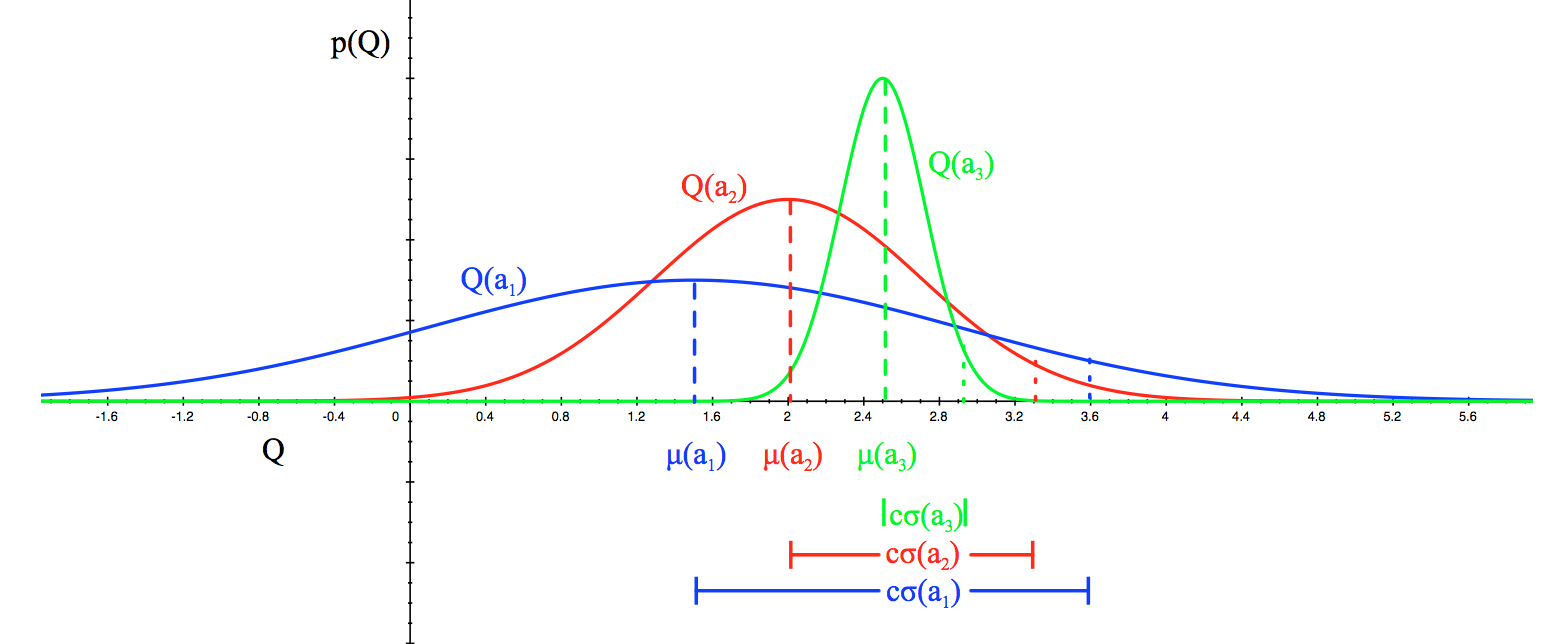
\includegraphics[height=1.5in]{figs/silver-UCB}
\caption{
Illustration of the reward distribution $Q(a)$
for a Gaussian bandit with 3 different actions,
and the corresponding lower and upper confidence bounds.
We show the posterior means $Q(a) = \mu(a)$ with a vertical
dotted line, and the scaled posterior standard deviations $c \sigma(a)$
as a horizontal solid line.
  \figtaken{\citep{Silver2018L9}}.
\figthanks{David Silver}.
}
\label{fig:UCB}
\end{figure}


\subsubsection{MDP case}

The UCB idea (especially in its frequentist form)
has been extended to the MDP case in several works.
(The Bayesian version is discussed in \cref{sec:thompson}.)
For example, \citep{Auer2002}
proposes to combine UCB with Q learning, by defining the policy as
\be
\pi(a|s) = \ind{a = \argmax_{a'} Q(s,a')
  + c \sqrt{\log(t)/N_t(s,a')}}
\ee
\citep{Auer2008} presents the more sophisticated \keywordDef{UCRL2} algorithm,
which computes confidence intervals on all the MDP model
parameters at the start of each episode; it then computes the resulting
\keywordDef{optimistic MDP} and solves for the optimal policy,
which it uses to collect more data.
%They prove a regret bound for their method.
%and \citep{Bourel2020} present the
%\keywordDef{UCRL3} algorithm.

\eat{
(However, 
the Bayesian posterior sampling approach to MDPs,
discussed in \cref{sec:PSRL}, works much better,
both in theory and practice
\citep{Osband2013,osband2017posterior,Agrawal2017}.)
}


\subsection{Thompson sampling}
\label{sec:thompson}

A common alternative to UCB is to use
 \keywordDef{Thompson sampling}
\citep{Thompson1933},
also called  \keywordDef{probability matching} \citep{Scott10}.
We start by describing this in the bandit case,
then extend to the MDP case.
For more details, see \citep{Russo2018}.
(See also \citep{Gershman2018} for some evidence that humans use
Thompson-sampling like mechanisms.)

\subsubsection{Bandit case}

In Thompson sampling,
we define the policy at step $t$ to be
$\policy_t(a|s_t,\history_t) = p_a$,
where $p_a$ is  the probability that $a$ is the optimal action.
This can be computed using
\begin{align}
p_a &= \Pr(a=a_*|s_t,\history_t)
  = \int \ind{a = \argmax_{a'} R(s_t,a';\vtheta)}
  p(\vtheta|\history_t) d\vtheta
  \label{eqn:bandit-probmatching}
\end{align}
If the posterior is uncertain, the agent will sample many different
actions, automatically resulting in exploration.
As the uncertainty decreases, it will start to exploit its knowledge.

To see how we can implement this method,
note that 
we can compute the expression
in \cref{eqn:bandit-probmatching} 
by using a single
Monte Carlo sample
$\tilde{\vtheta}_t \sim p(\vtheta|\history_t)$.
We then plug in this parameter
into our reward model, and greedily pick the best action:
\be
a_t = \argmax_{a'} R(s_t, a';\tilde{\vtheta}_t)
\ee
This sample-then-exploit approach
will choose actions with exactly
the desired probability, since
\begin{align}
  p_a
= \int \ind{a=\argmax_{a'} R(s_t,a';\tilde{\vtheta}_t)} p(\tilde{\vtheta}_t|\history_t) 
 = \Pr_{\tilde{\vtheta}_t \sim p(\vtheta|\history_t)}(a=\argmax_{a'} R(s_t, a';\tilde{\vtheta}_t)) 
\end{align}

Despite its simplicity,
this approach can be shown to
achieve optimal  regret (see e.g., \citep{Russo2018} for
a survey).
In addition, it is very easy to implement,
and hence is widely used  in practice~\citep{Graepel10,Scott10,Chapelle11}.

\begin{figure}
\centering
\begin{subfigure}[b]{0.3\textwidth}
\centering
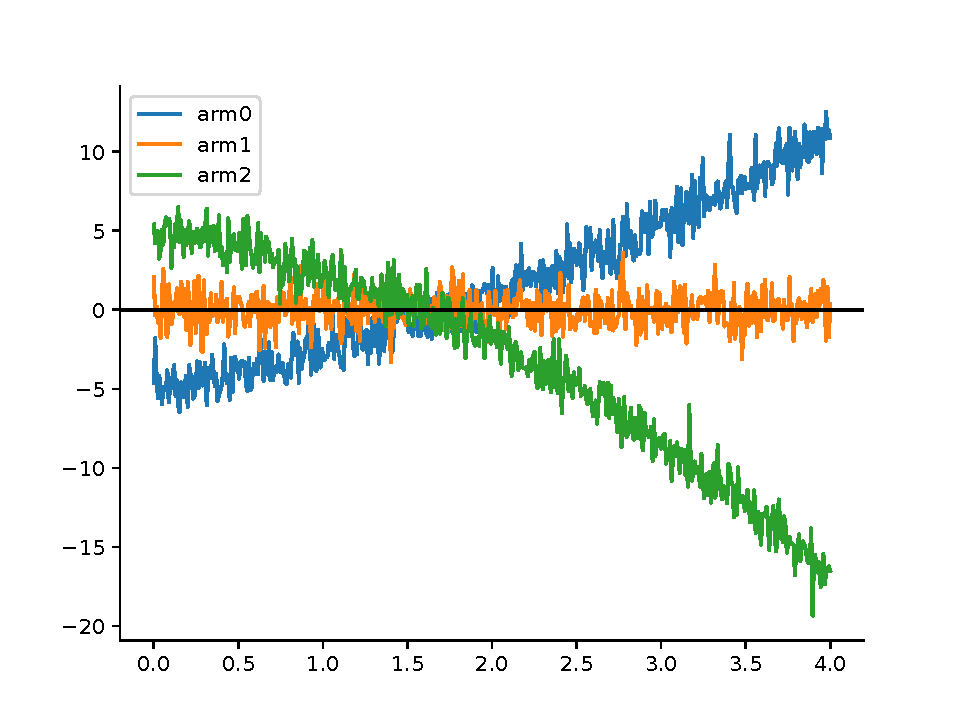
\includegraphics[height=1.5in]{figs/bandit-lingauss-true-reward}
\caption{ }
\end{subfigure}
~
\begin{subfigure}[b]{0.3\textwidth}
  \centering
  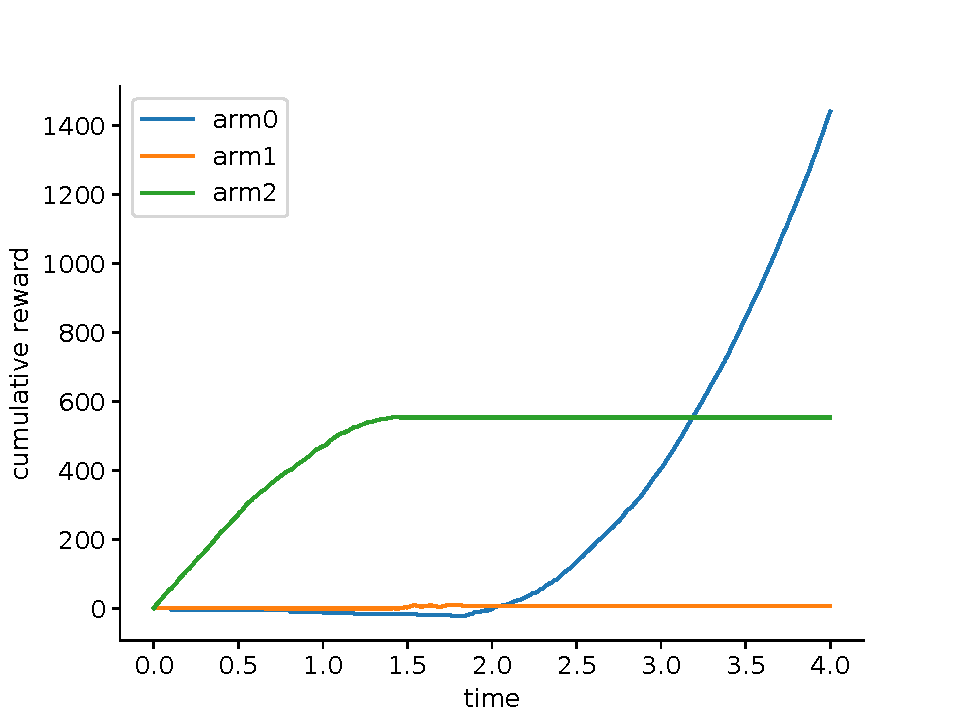
\includegraphics[height=1.5in]{figs/bandit-lingauss-cumulative-reward}
\caption{ }
\end{subfigure}
~
\begin{subfigure}[b]{0.3\textwidth}
  \centering
    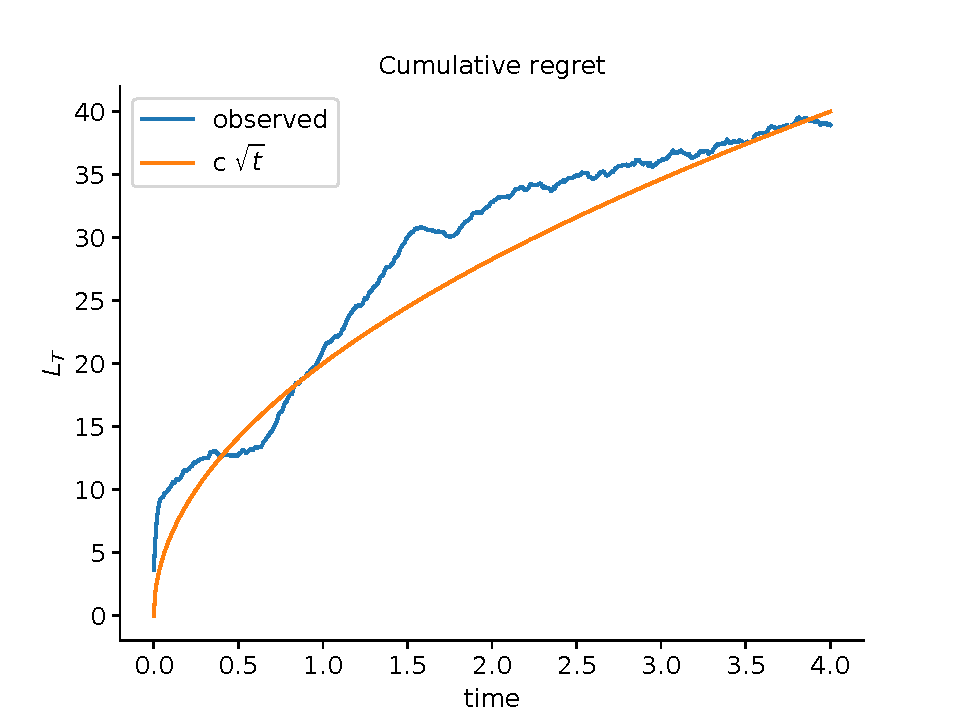
\includegraphics[height=1.5in]{figs/bandit-lingauss-cumulative-regret}
\caption{ }
\end{subfigure}
\caption{
  Illustration of Thompson sampling applied to a linear-Gaussian
  contextual bandit. The context has the form $\vs_t =(1,t,t^2)$.
  (a) True reward for each arm vs time.
  (b) Cumulative reward per arm vs time.
  (c) Cumulative regret vs time.
  \figgen{\notebook{thompson\_sampling\_linear\_gaussian}}.
}
\label{fig:banditsLingauss}
\end{figure}

In \cref{fig:banditsLingauss}, we give a simple
example of Thompson sampling applied to a linear regression bandit.
The context has the form $\vs_t =(1,t,t^2)$.
The true reward function has the form
$R(\vs_t,a) = \vw_a^\trans \vs_t$.
The weights per arm are chosen as follows:
$\vw_0 = (-5, 2, 0.5)$,
$\vw_1 = (0,0,0)$,
$\vw_2 = (5, -1.5, -1)$.
Thus we see that arm 0 is initially worse (large negative bias)
but gets better over time (positive slope),
arm 1 is useless,
and arm 2 is initially better (large positive bias)
but gets worse over time.
The observation noise is the same for all arms, $\sigma^2=1$.
See \cref{fig:banditsLingauss}(a) for a plot of the reward function.
We use a conjugate Gaussian-gamma prior and perform
exact Bayesian updating. Thompson sampling
quickly discovers that arm 1 is useless.
Initially it pulls arm 2  more,
but it adapts to the non-stationary nature of the problem
and switches over to arm 0,
as shown in 
\cref{fig:banditsLingauss}(b).
In \cref{fig:banditsLingauss}(c), we show that the empirical
cumulative regret in blue is close to the optimal
lower bound in red.

\subsubsection{MDP case (posterior sampling RL)}
\label{sec:PSRL}

We can generalize Thompson sampling to the (episodic) MDP case
by maintaining a posterior over all the model parameters
(reward function and transition model),
sampling an MDP from this belief state at the start of each episode,
solving for the optimal policy
corresponding to the sampled MDP,
using the resulting policy to collect new data,
and then updating the belief state at the end of the episode.
This is called \keywordDef{posterior sampling RL}
\citep{Strens00,Osband2013,Russo2014,osband2017posterior,Wang2024}.



As a more computationally efficient alternative,
it is also possible to maintain a posterior over policies
or $Q$ functions instead of over world models;
see e.g., \citep{Osband2023TS} for an implementation of this idea
based on \keywordDef{epistemic neural networks}
\citep{Osband2023epi}.
Another approach is to use successor features (\cref{sec:SF}),
where the $Q$ function is assumed to have the form
$Q^{\pi}(s,a) = \vpsi^{\pi}(s,a)^\trans \vw$.
In particular, \citep{Janz2019} proposes
\keywordDef{Sucessor Uncertainties},
in which they model the uncertainty over $\vw$
as a Gaussian,
$p(\vw) = \gauss(\vmu_{\vw}, \vSigma_{\vw})$.
From this they can derive the posterior distribution
over $Q$ values as
\be
p(Q(s,a)) = \gauss(\vPsi^{\pi} \vmu_{\vw}, \vPsi^{\pi} \vSigma_{\vw} (\vPsi^{\pi})^\trans)
\ee
where $\vPsi^{\pi}=[\vpsi^{\pi}(s,a)]^\trans$ is a matrix of features,
one per state-action pair.


\section{RL as a posterior inference problem}
\label{sec:inferRL}
\label{sec:planningAsInference}
\label{sec:RLAI}


In this section, we discuss an approach to
policy optimization that reduces it
to probabilistic inference.
This is called \keywordDef{control as inference}
or \keywordDef{RL as inference},
and has been discussed in numerous works
(see e.g., \citep{Attias03,Toussaint06,Toussaint09Robot,Ziebart2010,
  Rawlik2012,Botvinick2012,Kappen2012,Hoffmann2017control,Levine2018inf,Watson2021}).
The resulting framework also forms the foundation
of the SAC method discussed in \cref{sec:SAC},
the MPO discussed in \cref{sec:MPO},
and the MPC method discussed in \cref{sec:SMCMPC}.

\subsection{Modeling assumptions}

% Watson2021
% %https://github.com/JoeMWatson/input-inference-for-control

\begin{figure}
\centering
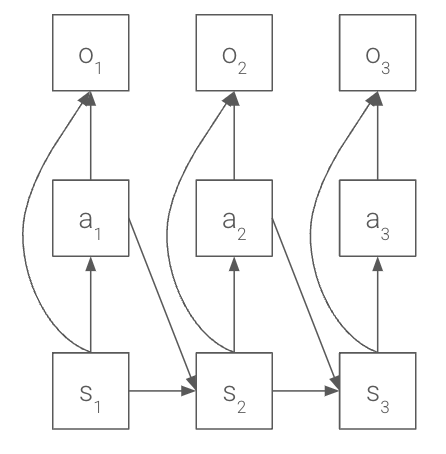
\includegraphics[height=2in]{figs/RLAIdieterich.png}
\caption{
  A graphical model for optimal control.
}
\label{fig:levine-rl-pgm}
\end{figure}

\cref{fig:levine-rl-pgm} gives a probabilistic model,
which not only captures state transitions as in a standard MDP,
but also introduces a new variable, $\optimality_t$.
This variable is binary, indicating whether the action at time $t$ is optimal or not, and has the following probability distribution:
\begin{align}
\label{eqn:merl-opt-prob}
p(\optimality_t=1 | s_t,a_t) = \exp( R(s_t,a_t))
\end{align}
In the above, we have assumed 
that $R(s,a) < 0$,
so that \cref{eqn:merl-opt-prob} gives a valid probability.
However, this is not required, since we can simply replace the
likelihood term
$p(\optimality_t=1 | s_t,a_t)$
with an unnormalized potential, $\phi_t(s_t,a_t)$;
this will not affect the results of inference.
For brevity, we will just write $p(\optimality_t)$
rather than $p(\optimality_t=1)$, since 1 is just a dummy value.


To simplify notation, we assume a
uniform action prior, $p(a_t|s_t)=1/|\calA|$;
this is without loss of generality,  since we can always push
an informative action prior $p(a_t|s_t)$ into the potential function $\phi_t(s_t,a_t)$.
(We call this an ``action prior'' rather than a policy, since we are going
to derive the policy using posterior inference, as we explain below.)
Under these assumptions, the  posterior probability
of observing a length-$T$ trajectory $\traj$, when optimality achieved in every step, is
\begin{align}
p(\traj | \voptimality_{1:T})
\propto p(\traj, \voptimality_{1:T})
&\propto \left[
p(s_1)  \prod_{t=1}^{T-1} \ptran(s_{t+1}|s_t,a_t)\right]
\left[\prod_{t=1}^{T} p(\optimality_t|s_t,a_t)\right]  \notag \\
&= p(s_1) \prod_{t=1}^{T-1} \ptran(s_{t+1}|s_t,a_t)
\exp\left(\sum_{t=1}^{T} R(s_t,a_t)\right)
\label{eqn:rl-merl-trajprob}
\end{align}
(Typically $p(s_1)$ is a delta function at the observed initial state $s_1$.)
The intuition of \cref{eqn:rl-merl-trajprob} is clearest when the state transitions are deterministic.
In this case, $\ptran(s_{t+1}|s_t,a_t)$ is either $1$ or $0$,
depending on whether the transition is dynamically feasible or not.
Hence we have
\be
p(\traj | \voptimality_{1:T})
\propto \ind{p(\traj) \neq 0} \exp(\sum_{t=1}^{T} R(s_t,a_t))
\ee
where the first term determines if $\traj$ is feasible or not.
In this case, find the action sequence that maximizes
the sum of rewards is equivalent to inferring the MAP sequence of actions,
which we denote by $\hat{\va}_{1:T}(s_1)$.
(The case of stochastic transitions is more complicated, and will be discussed later.)

For deterministic environments, the optimal policy is \keywordDef{open loop},
and corresponds to following the optimal action sequence $\hat{\va}_{1:T}(s_1)$.
(This is like a shortest path planning problem.)
However, in the stochastic case, we need to compute a \keywordDef{closed loop} policy,
$\pi(a_t|s_t)$,
that conditions on the observed state.
To compute this, let us define the following quantities:
\begin{align}
  \beta_t(s_t,a_t) &\defeq  p(\voptimality_{t:T}|s_t,a_t)\\
  \beta_t(s_t) &\defeq  p(\voptimality_{t:T}|s_t)
\end{align}
(These terms are
analogous to the \keywordDef{backwards messages} in the forwards-backwards algorithm
for HMMs \citep{Rabiner89}.)
Using this notation,
we can write the optimal policy using
\begin{align}
  p(a_t|s_t,\voptimality_{t:T}) &=
  \frac{p(s_t,a_t|\voptimality_{t:T})}{p(s_t|\voptimality_{t:T})}
  = \frac{p(\voptimality_{t:T}|s_t,a_t)p(a_t|s_t)p(s_t)}
  {p(\voptimality_{t:T}|s_t)p(s_t)} 
 \propto \frac{\beta_t(s_t,a_t)}{\beta_t(s)}
\label{eqn:rl-merl-optimal}
\end{align}
We can compute the backwards messages as follows:
\begin{align}
  \beta_t(s_t,a_t) &= 
  \int_\calS \beta_{t+1}(s_{t+1})
  \ptran(s_{t+1}|s_t,a_t) p(\optimality_t|s_t,a_t) ds_{t+1} \\
  \beta_s(s_t) &= \int_\calA \beta_t(s_t,a_t) p(a_t|s_t) da_t
\propto \int_\calA \beta_t(s_t,a_t) da_t  
\end{align}
where we have assumed the action prior $p(a_t|s_t) = 1/|\calA|$
for notational simplicty.
(Recall that the action prior is distinct from the optimal policy,
which is given by $p(a_t|s_t,\voptimality_{t:T})$.)

\subsection{Soft value functions}

We can gain more insight into what is going on by working in log space.
Let us define
\begin{align}
  Q(s_t,a_t) &= \log \beta_t(s_t,a_t) \\
  V(s_t) &= \log \beta_t(s_t)
\end{align}
The update for $V$ becomes
\be
V(s_t) = \log \sum_{a_t} \exp(Q(s_t,a_t)) 
\ee
This is a standard log-sum-exp computation,
and is similar to the softmax operation.
Thus we call it a \keywordDef{soft value function}.
When the values of $Q(s_t,a_t)$ are large
(which can be ensure by scaling up all the rewards),
this approximates the standard hard max operation:
\be
V(s_t) = \log \sum_{a_t} \exp(Q(s_t,a_t))
\approx \max_{a_t} Q(s_t,a_t)
\ee
For the deterministic case, the backup for $Q$ becomes
the usual
\be
Q(s_t,a_t) =  \log p(\optimality_t|s_t,a_t)
+ \log \beta_{t+1}(s_{t+1}) 
= r(s_t,a_t) + V(s_{t+1})
\ee
where $s_{t+1}=f(s_t,a_t)$ is the next state.
However, for the stochastic case, we get
\be
Q(s_t,a_t) = r(s_t,a_t) + \log \expectQ{\exp(V(s_{t+1}))}{\ptran(s_{t+1}|s_t,a_t)}
\ee
This replaces the standard expectation over the next state
with a softmax. This can result in Q functions that are optimistic,
since if there is one next state with particularly high reward
(e.g., you win the lottery), it will dominate the backup,
even if on average it is unlikely.
This can result in risk seeking behavior,
and is known as the \keywordDef{optimism bias}
(see e.g., \citep{Maddison2017,Chan2021} for discussion).
We will discuss a solution to this below.

\subsection{Maximum entropy RL}
\label{sec:maxentRL}


Recall that the true posterior is given by 
\begin{align}
  p(\traj | \voptimality_{1:T})
\defeq p^*(\traj)  
&\propto p(s_1) \prod_{t=1}^{T-1} \ptran(s_{t+1}|s_t,a_t)
\exp\left(\sum_{t=1}^{T} R(s_t,a_t)\right)
\end{align}
In the sections above, we derived
the exact posterior over states and actions conditioned
on the optimality variables.
However, in general we will have to approximate it.

Let us denote the approximate posterior by $q(\traj)$.
Variational inference corresponds to the minimizing (wrt $q$)
the following objective:
\be
\KLpq{q(\traj)}{p^*(\traj)}
= -\expectQ{\log p^*(\traj) - \log q(\traj)}{q(\traj)}
\ee
We can drive this loss to its minimum value of 0
by performing exact inference,
which sets $q(\traj)=p^*(\traj)$,
which is given by
\be
p^*(\traj) = p(s_1|\voptimality_{1:T})
\prod_{t=1}^{T-1} \ptran(s_{t+1}|s_t,a_t,\voptimality_{1:T})
p(a_t|s_t,\voptimality_{1:T}))
\ee
Unfortunately, this uses an optimistic form
of the dynamics, $\ptran(s_{t+1}|s_t,a_t,\voptimality_{1:T})$,
in which the agent plans assuming it directly controls
the state distribution itself, rather than just the action distribution.
We can solve this optimism bias problem by instead using
a ``causal'' variational posterior of the following form:\footnote{
%
Unfortunately, this trick is specific to variational
inference, which means that other posterior inference
methods, such as sequential Monte Carlo
\citep{Piche2019,Lioutas2022},
will still suffer from the optimism bias in the stochastic case
(see e.g., \citep{Maddison2017} for discussion).
} %
\be
q(\traj)
= p(s_1)
\prod_{t=1}^{T-1} \ptran(s_{t+1}|s_t,a_t)
p(a_t|s_t,\voptimality_{1:T})
= p(s_1)
\prod_{t=1}^{T-1} \ptran(s_{t+1}|s_t,a_t)
\pi(a_t|s_t)
\ee
where $\pi(a_t|s_t)$ is the policy we wish to learn.
In the case of deterministic transitions,
where  $\ptran(s_{t+1}|s_t,a_t)=\delta(s_{t+1}-f(s_t,a_t))$,
we do not need this simplification,
since  $\ptran(s_{t+1}|s_t,a_t,\voptimality_{1:T})
=\ptran(s_{t+1}|s_t,a_t)$.
(And in both cases $p(s_1|\voptimality_{1:T})=p(s_1)$,
which is assumed to be a delta function.)
We can now write the 
 (negative of) the objective as follows:
\begin{align}
  -\KLpq{q(\traj)}{p^*(\traj)}
  &= \E_{q(\traj)} \left[
    \log p(s_1) + \sum_{t=1}^T
    \left( \log \ptran(s_{t+1}|s_t,a_t) + R(s_t,a_t) \right) - \right. \\
    & \left.
        -\log p(s_1) - \sum_{t=1}^T
        \left( \log \ptran(s_{t+1}|s_t,a_t) + \log \pi(a_t|s_t) \right)
        \right] \\
  &= \E_{q(\traj)} \left[ \sum_{t=1}^T R(s_t,a_t)- \log \pi(a_t|s_t) \right] \\
  &= \sum_{t=1}^T \E_{q(s_t,a_t)}[R(s_t,a_t)]
  + \E_{q(s_t)} \entropy(\pi(\cdot|s_t))
  \label{eqn:maxentRL}
  \end{align}
This is known as the \keywordDef{maximum entropy RL} objective
\citep{Ziebart2010}.%,SAC,Haarnoja2018SAC}
We can optimize this using the
\keyword{soft actor critic} algorithm
which we discuss in \cref{sec:SAC}.

Note that we can tune the magnitude of the entropy regularizer
by defining the optimality variable using
$p(\optimality_t=1|s_t,a_t) = \exp(\frac{1}{\alpha} R(s_t,a_t))$.
This gives the objective
\begin{align}
  J(\pi)
  &= \sum_{t=1}^T \E_{q(s_t,a_t)}[R(s_t,a_t)]
  + \alpha \E_{q(s_t)} \entropy(\pi(\cdot|s_t))
\end{align}
As $\alpha \ra 0$ (equivalent to scaling up the rewards),
this approaches the standard
(unregularized) RL objective.



\eat{

The calculation above is expensive.
In practice,
we can approximate the optimal policy using a parametric form, $\policy_\theta(a_t|s_t)$.
The resulting probability of trajectory $\traj$ now becomes
\begin{align}
p_\theta(\traj) = p(s_0) \prod_{t=1}^{T} \ptran(s_{t+1}|s_t,a_t) \policy_\theta(a_t|s_t)
\end{align}
We now optimize $\theta$ so that $\KLpq{p_\theta(\traj)}{p(\traj|\voptimality_{1:T}=\vone)}$
is minimized, which gives the following objective
(where we push all terms that are independent of $\vtheta$ into the constant):
\begin{align}
\label{eqn:rl-merl-klobj}
\KLpq{p_\theta(\traj)}{p(\traj|\voptimality_{1:T})}
= -\expectQ{\sum_{t=1}^{T} \lambda^{-1} R(s_t,a_t) + \entropy(\policy_{\vtheta}(s_t))}{p_\theta} + \const
\end{align}
In other words, the objective is to maximize total reward,
with an entropy regularization favoring more uniform policies.
Thus this approach is called
\keywordDef{maximum entropy RL},
or \keywordDef{MERL}.


If $\polapprox$ can represent all stochastic policies,
a softmax version of the Bellman equation
can be obtained for \cref{eqn:rl-merl-klobj}:
\begin{align}
  \Qopt(s_t,a_t) = \lambda^{-1} R(s_t,a_t) +
  \expectQ{\log\int_\calA\exp(\Qopt(s_{t+1},a_{t+1}))da}{\ptran(s_{t+1}|s_t,a_t)}
\end{align}
with the convention that $\Qopt(s_T,a) = 0$ for all $a$,
and the optimal policy has a softmax form:
$\polopt(a_t|s_t) \propto \exp(\Qopt(s_t,a_t))$.
Note that the $\Qopt$ above is different from
the usual optimal $Q$-function (\cref{eqn:bellmanOptQ}),
due to the introduction of the entropy term.
However, as $\lambda \to 0$, their difference vanishes,
and the softmax policy becomes greedy,
recovering the standard RL setting.
}



\subsection{Active inference}

Control as inference is closely related
to a technique known as \keywordDef{active inference},
as we explain below. For more details on the connection, see
\citep{Millidge2020,Watson2020,VanDeLaar2021,Sajid2021,Tschantz2020}.

The active inference technique was developed in the neuroscience
community, that has its own vocabulary for standard ML concepts.
We start with 
the \keywordDef{free energy principle} 
 \citep{Friston2009,Buckley2017,Schwobel2018,
  Gershman2019,Mazzaglia2022}.
The FEP is equivalent to using variational  inference
to perform state estimation (perception)
and parameter estimation (learning)
in a latent variable model.
In particular, consider an LVM $p(\vz,\vo|\vtheta)$
with hidden states $\vz$, observations $\vo$, and parameters
$\vtheta$. 
We define the \keyword{variational free energy} to
be
\be
\calF(\vo|\vtheta)
= \KLpq{q(\vz|\vo,\vtheta)}{p(\vz|\vo,\vtheta)} - \log p(\vo|\vtheta)
= \expectQ{\log q(\vz|\vo,\vtheta) - \log p(\vo,\vz|\vtheta)}
{q(\vz|\vo,\vtheta)}
\geq -\log p(\vo|\vtheta)
\ee
which is the KL between the approximate variational posterior $q$
and the true posterior $p$, minus a normalization constant,
$\log p(\vo|\vtheta)$, which is known as the free energy.
State estimation (perception) corresponds to solving
$\min_{q(\vz|\vo,\vtheta)} \calF(\vo|\vtheta)$,
and parameter estimation (model fitting)
corresponds to solving $\min_{\vtheta} \calF(\vo|\vtheta)$,
just as in the  EM (expectation maximization) algorithm.
(We can also be Bayesian about $\vtheta$,
as in variational Bayes EM,
instead of just
computing a point estimate.)
This EM procedure will minimize the VFE,
which is an upper bound on the negative log marginal likelihood of the
data. In other words, it adjusts the model (belief state
and parameters) so that it better
predicts the observations, so the agent is less surprised
(minimizes prediction errors).



To extend the above FEP to decision making problems,
we define the \keywordDef{expected free energy}
as follows
\be
\calG(\va) 
%\overline{\calF}(\va)
= \expectQ{\calF(\vo)}{q(\vo|\va)}
= \expectQ{\log q(\vz|\vo) - \log p(\vo,\vz)}{q(\vo,\vz|\va)}
\ee
where $q(\vo|\va)$ is the posterior predictive distribution
over future observations given action sequence $\va$.
(We can also condition on any observed  history or agent state $\vh$,
but we omit this (and the model parameters $\vtheta$) from the notation for brevity.)
We can decompose the EFE (which the agent wants to minimize)
into two terms.
First there is the \keywordDef{intrinsic value},
known as the \keywordDef{epistemic drive}:
\be
\calG_{\text{epistemic}}(\va) = \expectQ{\log q(\vz|\vo) - \log q(\vz)}{q(\vo,\vz|\va)}
\ee
Minimizing this will encourage the agent to choose actions
which maximize the mutual information between
the observations $\vo$ and the hidden states $\vz$,
thus reducing uncertainty about the hidden states.
(This is called \keywordDef{epistemic foraging}.)
%result in observations which cause the conditional
%posterior to match the prior
The \keywordDef{extrinsic value},
known as the \keywordDef{exploitation term},
is given by
\be
\calG_{\text{extrinsic}}(\va) = -\expectQ{\log p(\vo)}{q(\vo|\va)}
\ee
Minimizing this will encourage the agent to choose actions
that result in observations that match its prior.
For example, if the agent predicts that the world will look brighter
when it flips a light switch, it can take the action of flipping
the switch to fulfill this prediction.
This prior can be related to a reward function by defining
as $p(\vo) \propto e^{R(\vo)}$, encouraging goal directed behavior,
exactly as in control-as-inference.
However, the active inference approach provides
a way of choosing actions without needing to specify a reward.
Since solving to the optimal action at each step can be slow,
it is possible to amortize this cost by training a policy network to compute
$\pi(\va|\vh) = \argmin_{\va} \calG(\va|\vh)$,
where $\vh$ is the observation history (or current state),
as shown in \citep{Millidge2020vpg,van-der-Himst2020};
this is called \keywordDef{``deep active inference''}.


Overall, we see that this framework
provides a unified theory of both perception and action,
both of which try to minimize some form of free energy.
In particular, minimizing the expected free energy will cause
the agent to pick actions to reduce its uncertainty about its hidden states,
which can then be used to improve its predictive model $p_\vtheta$
of observations; this in turn will help minimize the VFE of future observations,
by updating the internal belief state $q(\vz|\vo,\vtheta)$
to explain the observations.
In other words,
the agent acts so it can learn so it becomes less surprised
by what it sees.
This ensures the agent is in \keywordDef{homeostasis} with its environment.



\eat{
To guide the agent towards preferred outcomes (beyond just information seeking),
we define the prior over states as $p(\vz) \propto e^{R(\vz)}$,
where $R$ is the reward function.
Alternatively, we can define the prior over observations
as $p(\vo) \propto e^{R(\vo)}$.
Either way, the prior
is defined in terms of what the agent
wants to achieve, rather than being an ``objective'' model of reality
(c.f., optimism bias in control-as-inference mentioned above).
\eat{
The advantage of this approach is that it automatically
induces  {\em goal-directed} information-seeking
behavior, rather than than the maxent approach which models
uncertainty in a goal-independent way.
Hence the term ``active inference''.
}
}

Note that active inference is often discussed in the context of
\keywordDef{predictive coding}.
This is equivalent to a special case of FEP
where two assumptions are made:
(1)  the generative model $p(\vz,\vo|\vtheta)$ is a 
a  nonlinear hierarchical Gaussian  model
(similar to a VAE decoder),
and (2) the variational posterior approximation
uses a diagonal Laplace approximation,
$q(\vz|\vo,\vtheta) =\gauss(\vz|\hat{\vz},\vH)$
with the mode $\hat{\vz}$
being computed using gradient descent, and $\vH$ being the Hessian
at the mode.
This can be considered a non-amortized version of a VAE,
where inference (E step) is done with iterated gradient descent,
and parameter estimation (M step) is also done with gradient descent.
(A more efficient incremental EM version of predictive
coding, which updates $\{ \hat{\vz}_n: n=1:N\}$ and $\vtheta$ in parallel,
was recently presented in \citep{Salvatori2024iclr},
and an amortized version in \citep{Tscshantz2023}.)
For more details on predictive coding,
see
\citep{Rao1999predictive,Friston2003,Spratling2017,Hosseini2020pc,
  Millidge2021pc,Marino2021,Ororbia202,Salvatori2023,Salvatori2024iclr}.
%https://github.com/NACLab/ngc-learn

